\section{Metric Spaces}
\begin{defn}[Metric Space \cite{fa2019}]\label{defn:metric_space}
	Let $X$ be a non-empty set. Then the map 
	\begin{align*}
		d: X\times X\rightarrow \mathbb R
	\end{align*}
	is called a \textit{metric} on $X$ if for all $\varphi$, $\psi$, $\chi\in X$ the following properties are given: 
	\begin{itemize}
		\item \textbf{positivity}: $d(\varphi, \psi) \geq 0$, 
		\item \textbf{symmetry}: $d(\varphi, \psi) = d(\psi, \varphi)$, 
		\item \textbf{definiteness}: $d(\varphi, \psi) = 0$ iff $\varphi = \psi$, 
		\item \textbf{triangle inequality}: $d(\varphi, \psi) \leq d(\varphi, \chi) + d(\chi, \psi)$. 
	\end{itemize}
\end{defn}

\begin{theorem}
	Let $X$ be a linear space and $d$ a metric on $X$. Then $\norm{x}{} := d(x, 0)$ defines a norm on $X$ if $d(tx, 0) = \abs{t}d(x, 0)$ (\enquote{scaling property}) for all $t\in\mathbb K$, $x\in X$, and if $d(x + y, y) = d(x, 0)$ for all $x, y\in X$ (\enquote{translation invariance}).
\end{theorem}

\begin{proof}
	Positivity, definiteness and homogeneity of $\norm{\cdot}{}$ are obvious, for the triangle inequality note that for all $x, y\in X$,
	\begin{align*}
		\norm{x + y}{} &= d(x + y, 0) = d(x, -y) \leq d(x, 0) + d(0, -y) = d(x, 0) + d(-y, 0) 
		\\ &= d(x, 0) + d(y, 0) = \norm{x}{} + \norm{y}{}.
	\end{align*}
\end{proof}

\begin{theorem}\label{thrm:new_metric_out_of_given_metric}
	Let $(X, d)$ be a metric space, then $(X, \rho)$ with 
	\begin{align}
		\rho(x, y) := \frac{d(x, y)}{1 + d(x, y)}
	\end{align}
	for all $x, y\in X$ is also a metric space.
\end{theorem}

\begin{proof}[Proof \cite{1860725, 686797}]
	Clearly, $\rho$ is positive and symmetric. If $\rho(x, y) = 0$, then this is only possible iff $d(x, y) = 0$, which is equivalent to $x = y$, i.e. $\rho$ is also definite. For the triangle inequality, first note that for all $a, b\in\mathbb R_{\geq 0}$ with $a\in [0, b]$, we have
	\begin{align}\label{eq:inequality_reals_intermed_step}
		\frac{a}{1 + a} \leq \frac{b}{1 + b}.
	\end{align} 
	If $a = 0 = b$ or $a = 0$ and $b > 0$, then the inequality trivially holds. Thus, assume $a, b\ne 0$. Then
	$$\frac{a}{1 + a} = \frac{1}{\frac{1}{a} + 1} \leq \frac{1}{\frac{1}{b} + 1} = \frac{b}{1 + b},$$ since $b\geq a$. Thus, for any $x, y, z\in X$, we have
	\begin{align*}
		\rho(x, y) &= \frac{d(x, y)}{1 + d(x, y)} \overset{\tiny\eqref{eq:inequality_reals_intermed_step}}{\leq} \frac{d(x, z) + d(z, y)}{1 + d(x, z) + d(z, y)} 
		\\ &= \frac{d(x, z)}{1 + d(x, z) + d(z, y)} + \frac{d(z, y)}{1 + d(x, z) + d(z, y)}
		\\ &\leq \frac{d(x, z)}{1 + d(x, z)} + \frac{d(z, y)}{1 + d(z, y)} 
		\\ &= \rho(x, z) + \rho(z, y).
	\end{align*}
\end{proof}

\begin{remark}
	The metric $\rho$ from Theorem \ref{thrm:new_metric_out_of_given_metric} is bounded between $0$ and $1$, $\rho(x, y) \in [0, 1)$ for all $x, y\in X$.
\end{remark}

\begin{theorem}\label{thrm:vierecksungleichung}
	Let $(X, d)$ be a metric space. Then we have the inequality
	\begin{align}
		\abs{d(\varphi, \psi) - d(\varphi', \psi')} \leq d(\varphi, \varphi') + d(\psi, \psi') \quad \forall \varphi, \varphi', \psi, \psi'\in X.
	\end{align}
\end{theorem}

\begin{proof}
	Let $\varphi, \varphi', \psi, \psi'\in X$ be arbitrary. Applying the triangle inequality twice, we have
	\begin{align}
		d(\varphi, \psi) \leq d(\varphi, \varphi') + d(\varphi', \psi) &\leq d(\varphi, \varphi') + d(\psi, \psi') + d(\psi', \varphi')
		\\ \Rightarrow d(\varphi, \psi) - d(\varphi', \psi') &\leq d(\varphi, \varphi') + d(\psi, \psi')
	\end{align}
	Exchanging the roles of $\varphi$ and $\varphi'$ and $\psi$ and $\psi'$, we get the stated inequality.
\end{proof}

\begin{remark}[Discrete Metric]\label{remark:discrete-metric}
	Let $X$ be an arbitrary set and $d(\varphi, \psi) = 1 \ \forall \varphi$, $\psi\in X$ and $d(\varphi, \varphi) = 0$. Then $d$ is a metric, called the \textit{discrete metric} on $X$. 
\end{remark}

\begin{defn}[Open Ball]
	Let $(X, d)$ be a metric space, $\varphi\in X$ and $r > 0$. Then 
	\begin{align}
		B_{r}(\varphi) := \left\{ \psi\in X \vert d(\varphi, \psi) < r\right\} \subset X
	\end{align}
	is called an \textit{open ball} in $X$ with middle point $\varphi$ and radius $r$. 
\end{defn}

\begin{exmp}\label{exmp:open-balls-discrete-metric}
	For the discrete metric $d$ according to Remark \ref{remark:discrete-metric}, the open balls can be characterized as follows:
	\begin{align}
		B_{r}(\varphi) = \begin{cases}
			\{\varphi\}, &r \leq 1 
			\\ X, &r > 1
		\end{cases}
	\end{align}
\end{exmp} 

\begin{theorem}\label{thrm:intersection_open_balls}
	Let $(X, d)$ be a metric space, and $B_{\tilde{r}}(\tilde{x})$ and $B_{r'}(x')$ be open balls with $\tilde{x}, x'\in X$ and $\tilde{r}, r' > 0$. Then for all $x\in X$ with $x\in B_{\tilde{r}}(\tilde{x})\cap B_{r'}(x')$ there is an open ball containing $x$ and that is contained in $B_{\tilde{r}}(\tilde{x})\cap B_{r'}(x')$.
\end{theorem}

\begin{proof}[Proof \cite{886810}]
	The intuition of the proof is shown in Figure \ref{fig:open_balls_intersection}.
	\begin{figure}[h!]
		\centering
		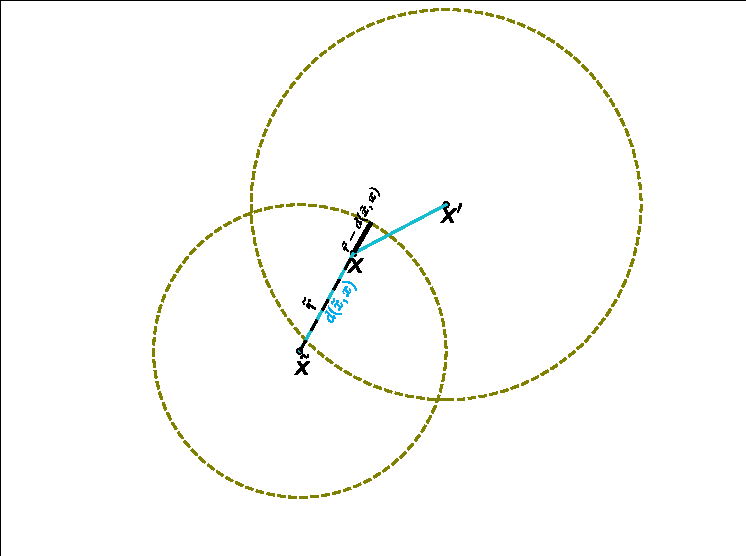
\includegraphics[trim={2.5cm 0.9cm 1.7cm 0.14cm}, clip, width=0.7\textwidth]{Figures/circles_modified.pdf}
		\caption{Any point in the intersection of two open balls lies in another open ball, which is contained in the intersection.}
		\label{fig:open_balls_intersection}
	\end{figure}
	If the intersection is empty, then the statement holds (vacuously). Let $x\in B_{\tilde{r}}(\tilde{x}) \cap B_{r'}(x')$, and thus $x\in B_{\tilde{r}}(\tilde{x})$ and $x\in B_{r'}(x')$. Define $r := \min\{ \tilde{r} - d(x, \tilde{x}), r' - d(x, x') \}$, and note that $x\in B_{r}(x)$. For all $y\in B_{r}(x)$, we have $d(y, \tilde{x}) \leq d(y, x) + d(x, \tilde{x}) < r + d(x, \tilde{x}) \leq \tilde{r}$, i.e. $y\in B_{\tilde{r}}(\tilde{x})$. Similarly, we can show $y\in B_{r'}(x')$, and thus $y\in B_{\tilde{r}}(\tilde{x})\cap B_{r'}(x')$, i.e. $B_{r}(x)\subset B_{\tilde{r}}(\tilde{x})\cap B_{r'}(x')$.
\end{proof}

\begin{defn}[Closed ball]
	Let $(X, d)$ be a metric space, $\varphi\in X$ and $r > 0$. Then 
	\begin{align}
		B_{r}[\varphi] := \left\{ \psi\in X \vert d(\varphi, \psi) \leq r\right\} \subset X
	\end{align}
	is called a \textit{closed ball} in $X$ with middle point $\varphi$ and radius $r$.
\end{defn}

\begin{defn}[Open Set]
	\label{defn-open-set}
	Let $(X, d)$ be a metric space. Then a subset $U\subset X$ is called \textit{open} in $X$ if for every $\varphi \in U$ there is an open ball $B_{r}(\varphi)$ that is contained in $U$, i.e. $B_r(\varphi)\subset U$. 
\end{defn}

\begin{defn}[Closed Set]
	Let $(X, d)$ be a metric space. Then a subset $A\subset X$ is called \textit{closed} in $X$ if the complement $X\backslash A$ is open according to Definition \ref{defn-open-set}. 
\end{defn}

\begin{theorem}\label{open-balls-open}
	Open balls are open. 
\end{theorem}

\begin{proof}
	An illustration of the idea of the proof is shown in Figure. 
	\begin{figure}[h!]
		\centering
		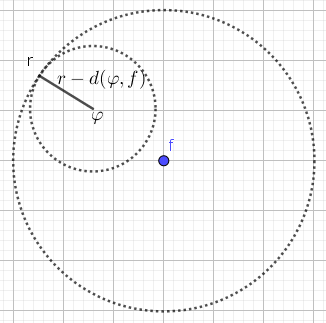
\includegraphics[width=0.35\textwidth]{Figures/open-balls-open.png}
	\end{figure}
	
	Let $f\in X$ and for $r > 0$ consider the open ball $U:= B_{r}(f) \subset X$. By definition, for every $\varphi \in U$ it holds that $d\left(\varphi, f\right) < r$. Now we show that 
	\begin{align}
		B_{r-d\left(\varphi, f\right)}(\varphi) \subset U.
	\end{align}
	For this consider $\psi\in B_{r-d\left(\varphi, f\right)}(\varphi)$, i.e. $d(\psi, \varphi) < r - d(\varphi, f)$. With the triangle inequality we obtain: 
	\begin{align}
		d(f, \psi) \leq d(f, \varphi) + d(\varphi, \psi) < d(f, \varphi) + r - d(\varphi, f) = r,  		
	\end{align}
	i.e. $d(f, \psi) < r$ and thus $\psi\in U = B_{r}(f)$.
\end{proof}


\begin{theorem}\label{thrm:closed_balls_open}
	Closed balls are closed.
\end{theorem}

\begin{proof}
	Let $f\in X$ and for $r > 0$ consider the closed ball $B_{r}[f]\subset X$. By definition, for every $\varphi \in X\backslash B_{r}[f]\subset X$, it holds that $d(\varphi, f) > r$. We will now show that 
	\begin{align}
		B_{d(\varphi, f) - r}(\varphi) \subset X \backslash B_{r}[f],
	\end{align}
	which would prove that $B_{r}[f]$ is closed. Let $\psi\in B_{d(\varphi, f) - r}(\varphi)$, i.e. $d(\psi, \varphi) < d(\varphi, f) -r$. With the triangle inequality, we obtain:
	\begin{align}
		d(f, \varphi) \leq d(f, \psi) + d(\psi, \varphi) \Leftrightarrow d(f, \psi) \geq d(f, \varphi) - d(\psi, \varphi) > d(f, \phi) - d(\varphi, f) + r = r, 
	\end{align}
	i.e. $d(f, \psi) > r$, and hence $\psi\notin B_r[f]$, implying that $\psi\in X\backslash B_{r}[f]$. 
\end{proof}

\begin{theorem}\label{thrm:open_sets_form_topology}
	Let $(X, d)$ be a metric space. The collection of open sets as in Definition \ref{defn-open-set} gives a topology.
\end{theorem}
\begin{proof}		
	According to Defn. \ref{defn:metric_space}, we need to prove that $X$ and $\emptyset$ are open, that the union of an arbitrary number of open sets is open, and that the intersection of a finite number of open sets is open. 
	
	Clearly, $X$ is open (since for any choice of $r > 0$ and $\varphi\in X$, $B_{r}(\varphi)\subset X$). $\emptyset$ is also open, since nothing needs to be shown.
	
	Now let $U_{1}$, $\dots$, $U_{n}\subset X$ be open, and consider the intersection
	\begin{align}
		U := \bigcap_{i=1}^{n}U_{i} \subset X.
	\end{align} 
	For any $\varphi\in U$, we know that $\varphi\in U_i$ for all $1\leq i \leq n$. Since the $U_{i}$ are open, there is a radius $r_{i} > 0$ such that $B_{r_i}(\varphi) \subset U_i$ for all $1\leq i \leq n$. Defining $r := \min_{1 \leq i \leq n}\{r_{i}\} > 0$, we have that $B_{r}(\varphi) \subset U_i$ for all $1\leq i\leq n$ and hence $B_{r}(\varphi)\subset U$.
	
	Finally, let $U_{i}$, $i\in I$, be open, where $I$ is in index set. Consider the union
	\begin{align}
		U := \bigcup_{i\in I}U_{i} \subset X.
	\end{align}
	For any $\varphi\in U$ there is an index $i\in I$ such that $\varphi\in U_i$. Since $U_i$ is open, there is an $r > 0$ such that $B_{r}(\varphi) \subset U_i \subset U$.
\end{proof}

\begin{defn}[Convergence of sequence \cite{fa2019}]\label{defn:convergence_sequence}
	Let $(X, d)$ be a metric space. A sequence $(\varphi_n)_{n\in\mathbb N}$ with elements $\varphi_n\in X$, $n\in\mathbb N$, is called \textit{convergent} if there is a $\varphi\in X$ s.t.
	\begin{align}
		\lim\limits_{n\to\infty}d(\varphi_n, \varphi) = 0,
	\end{align}
	i.e. for all $\epsilon > 0$ there exists an $N(\epsilon)\in\mathbb N$ s.t.
	\begin{align}
		d(\varphi_n, \varphi) < \epsilon \quad \forall n\geq N(\epsilon).
	\end{align}
	$\varphi$ is called the \textit{limit} of the sequence $(\varphi_n)_{n\in \mathbb N}$. For this, we write 
	\begin{align}
		\lim\limits_{n\to\infty}\varphi_n = \varphi \quad \text{or}\quad \varphi_n \overset{n \to\infty}{\longrightarrow} \varphi.
	\end{align}
	Non-convergent sequence are called \textit{divergent}.
\end{defn}

\begin{theorem}\label{thrm:sequences_unique_limits}
	Let $(X, d)$ be a metric space, and $\seq[\varphi_n]$ a convergent sequence in $X$ wrt $d$. Then the limit is unique.
\end{theorem}

\begin{proof}
	Assume the limit is not unique, i.e. $\seq[\varphi_n]$ converges to both $\varphi\in X$ and $\psi\in X$. with $\varphi\ne\psi$. Then for $\epsilon := d(\varphi, \psi) / 2$ there exists an $N'\in\mathbb N$ s.t. for all $n\geq N$, we have
	$$d(\varphi_n, \varphi) < \frac{d(\varphi, \psi)}{2} = \epsilon$$ 
	and an $\tilde{N}$ s.t. for all $n\geq \tilde{N}$, we have
	$$d(\varphi_n, \psi) < \frac{d(\varphi, \psi)}{2} = \epsilon.$$
	Define $N := \max\{N', \tilde{N}\}$, then for all $n\geq N$, we have
	$$d(\varphi, \psi) \leq d(\varphi, \varphi_n) + d(\varphi_n, \psi) < d(\varphi, \psi),$$
	which is a contradiction.
\end{proof}

\begin{theorem}\label{thrm:seq_convergence_subsequences}
	A sequence is convergent iff every subsequence converges to the same limit.
\end{theorem}

\begin{proof}[Proof \cite{213285}]
	\enquote{$\Longleftarrow$} Every sequence has a trivial subsequence, namely itself.
	
	\enquote{$\Longrightarrow$} Let $\left(\varphi_{n_k}\right)_{k\in\mathbb N}$ be a subsequence of $\seq[\varphi_n]$. Note that $n_k \geq k$ for all $k\in\mathbb N$, which we will prove by induction: Clearly, $n_1\geq 1$, and $n_k\geq k$ implies $n_{k + 1} > n_{k} \geq k$, i.e. $n_{k + 1}\geq k + 1$. 
	
	We denote the limit of $\seq[\varphi_n]$ by $\varphi$, and note that for all $\epsilon > 0$, there exists an $N\in\mathbb N$ s.t. for all $n \geq N$, we have $d(\varphi_n, \varphi) < \epsilon$. Thus, for all $k\geq N$ (and hence $n_k\geq N$), we have $d(\varphi_{n_k}, \varphi) < \epsilon$.
\end{proof}

\begin{defn}[Accumulation point]\label{defn:accumulation_point}
	Let $U\subset X$. Then $\varphi\in X$ is called an \textit{accumulation point} of $U$ if there is a sequence $\left(\varphi_{n}\right)_{n\in \mathbb N}$ in $U$ such that $\lim\limits_{n\to\infty}\varphi_{n} = \varphi$.
\end{defn}

\begin{theorem}\label{thm:closed_set_acc_point}
	A subset $U \subset X$ is closed if and only if it contains all its accumulation points according to Defn. \ref{defn:accumulation_point}.
\end{theorem}

\begin{proof}
	\enquote{$\Longleftarrow$}: Let $U$ contain all its accumulation points, and let $\varphi\in X\backslash U$. We will now show that there is an $n\in \mathbb N$ such that $B_{\frac{1}{n}}(\varphi) \subset X\backslash U$, proving that $X\backslash U$ is open. Assuming there is no such $n\in \mathbb N$, then $B_{\frac{1}{n}}(\varphi) \cap U = \emptyset$ for all $n\in \mathbb N$. This means that there is a sequence $(\varphi_{n})_{n\in\mathbb N}$ in $U$ such that $d(\varphi, \varphi_n) < \frac{1}{n}$ for all $n\in\mathbb N$. Hence, $\varphi$ is an accumulation point of $U$, and since $U$ contains all its accumulation points by assumption, it follows that $\varphi\in U$, contradicting the assumption that $\varphi\in X\backslash U$.
	
	\enquote{$\Longrightarrow$}: Let $U$ be closed, i.e. $X\backslash U$ is open. Further, let $\varphi\in X$ be an accumulation point of $U$, i.e. there is a sequence $(\varphi_n)_{n\in\mathbb N}$ in $U$ such that $\lim\limits_{n\to\infty}\varphi_n = \varphi$. Hence, by definition of convergence, for all $\epsilon > 0$ there exists an $n\in\mathbb N$ such that $\varphi_n\in B(\varphi, \epsilon) \cap U$, implying that $\varphi\in U$. Thus, $U$ contains all its accumulation points.
\end{proof}

\begin{corollary}\label{corollary:closed_bounded_subsets_contain_inf_sup}
	Let $U\subset \mathbb R$ be closed and bounded, where on $\mathbb R$ we consider the standard metric, then $\sup(U), \inf(U) \in U$, i.e. $\sup(U) = \max(U)$ and $\inf(U) = \min(U)$.
\end{corollary}

\begin{proof}[Proof \cite{2752236}]
	Since $U$ is bounded, $\inf(U)$ and $\sup(U)$ exist. 
	
	By Theorem \ref{thrm:supremum_characterization}, there exists a sequence $\seq[x_n]$ in $U$ s.t. $\sup(U) - \frac{1}{n} < x_n \leq \sup(U)$ for all $n\in\mathbb N$. Thus, $\lim\limits_{n\to\infty}x_n = \sup(U)$, i.e. $\sup(U)$ is an accumulation point of $U$ and since $U$ is closed, $\sup(U)\in U$.
	
	Similarly, one can show that $\inf(U)\in U$.
\end{proof}

\begin{defn}[Closure of set]\label{defn:closure_set}
	The set 
	\begin{align}
		\bar{U} := \{\varphi\in X\mid \varphi\ \text{is an accumulation point of}\ U\} \subset X
	\end{align}
	is called the closure of the set $U \subset X$.
\end{defn}

\begin{remark}\label{remark:closure_superset}
	Clearly, $U\subset \bar{U}$, since any $\varphi\in U$ is an accumulation point of $U$ (consider the constant sequence, where for any $n\in\mathbb N$, $\varphi_n := \varphi$).
\end{remark}

\begin{remark}
	According to Theorem \ref{thm:closed_set_acc_point}, a subset $U\subset X$ is closed if and only if it contains all its limit points, thus for a closed subset we have $\overline{U} \subset U$. With Remark \ref{remark:closure_superset}, we get $U$ is closed if and only if $U = \overline{U}$.
\end{remark}

\begin{theorem}\label{thrm:closure_closed}
	Let $U\subset X$. Then its closure, $\bar{U}$, is closed.
\end{theorem}

\begin{proof}
	According to Theorem \ref{thm:closed_set_acc_point}, we need to prove that $\bar{U}$ contains all its limit points. Let $\varphi\in X$ be an accumulation point of $\overline{U}$. Then for all $n\in \mathbb N$ there is a $\varphi_n\in\overline{U}$ such that $d(\varphi, \varphi_n) < 1/n$. By Def. \ref{defn:closure_set}, we also know that since $\varphi_n\in \bar{U}$, it is an accumulation point of $U$, i.e. for every $\varphi_n\in \overline{U}$ there is a $\psi_n\in U$ such that $d(\varphi_n, \psi_n) < 1/n$. Thus:
	\begin{align}
		d(\psi_n, \varphi) \leq d(\psi_n, \varphi_n) + d(\varphi_n, \varphi) < \frac{1}{n} + \frac{1}{n} \overset{n\to\infty}{\longrightarrow} 0,
	\end{align}
	i.e. $(\psi_n)_{n\in\mathbb N}$ is a sequence in $U$ that converges to $\varphi$, i.e. $\varphi$ is an accumulation point of $U$, hence $\varphi\in \bar{U}$.
\end{proof}

\begin{theorem}\label{thrm:property_metric_space}
	Let $(X, d)$ be a metric space. Then $\varphi\in \overline{U}$ for $U\subset X$ if and only if for every open set $O\subset X$ containing $\varphi$, $U\cap O\ne \emptyset$.
\end{theorem}

\begin{proof}
	\enquote{$\Longrightarrow$} Since $\varphi\in\overline{U}$, there exists a sequence $\left(\varphi_n\right)_{n\in\mathbb N}$ converging to $\varphi$ wrt $d$, i.e. for all $\epsilon > 0$ there exists an $N\in\mathbb N$ s.t. for all $n\geq N$, $d(\varphi_n, \varphi) < \epsilon$. Let $O\subset X$ be open, and let $\varphi\in O$. By definition, there exists an open ball $B_{r}(\varphi)\subset O$ with $r > 0$. Choose $\epsilon = r$ and $\psi = x_{N}\in U$, then $\psi\in B_{r}(\varphi) \subset O$.
	
	\enquote{$\Longleftarrow$} By assumption, for any non-empty open set $O\subset X$, $U\cap O\ne\emptyset$, where $U\subset X$. Let $\varphi\in X$. Since open balls are open, for any $\epsilon > 0$, $U\cap B_{\epsilon}(\varphi)\ne\emptyset$. Consider the sequence of open balls $\left( B_{1/n}(\varphi)\right)_{n\in\mathbb N}$, for which $U\cap B_{\frac{1}{n}}(\varphi) \ne \emptyset$ holds. Thus for each $n\in\mathbb N$, there exists a point $\varphi_{n}\in X$ s.t. $\varphi_n \in B_{\frac{1}{n}}(\varphi)$ and $\varphi_n\in U$. Hence, by definition, $\varphi\in X$ is an accumulation point of $U$.
\end{proof}

\begin{theorem}
	Let $U\subset X$. Then its closure, $\overline{U}$, is the \textit{smallest} closed set in $X$ containing $U$.
\end{theorem}

\begin{proof}
	From Remark \ref{remark:closure_superset}, we know that $U\subset \overline{U}$, and from Theorem \ref{thrm:closure_closed}, we know that $\overline{U}$ is closed. To prove that $\overline{U}$ is the smallest \textit{closed} set in $X$ containing $U$, let $V\subset X$ be another closed set that contains $U$, i.e. $U\subset V$. Every sequence in $U$ is also a sequence in $V$, i.e. every accumulation point of $U$ is in $V$, i.e. $\overline{U}\subset V$.
\end{proof}

\begin{defn}[Bounded set]\label{defn:bounded_set}
	A subset $U\subset X$ is called \textit{bounded} in $X$ if it is contained in a closed ball in $X$, i.e. there exists $r > 0$ and $\varphi \in X$ s.t. $U\subset B_{r}[\varphi]$.
\end{defn}

\begin{theorem}
	Convergent sequences in $X$ are fully contained in a bounded subset.
\end{theorem}

\begin{proof}
	Let $(\varphi_n)_{n\in\mathbb N}$ be a convergent sequence in $X$ with limit point $\varphi\in X$. Then there exists an $N\in\mathbb N$ s.t. $d(\varphi_n, \varphi) < \epsilon$ for all $n\geq N$ for a fixed $\epsilon > 0$. Defining
	\begin{align}
		r := \max \left\{ \epsilon, \max_{n \leq N}\{d(\varphi, \varphi_n)\} \right\},
	\end{align}
	we have $d(\varphi, \varphi_n) \leq r$ for all $n\in\mathbb N$. Hence, for any $n\in\mathbb N$, 
	$\varphi_n\in B_{r}[\varphi]$.¸
\end{proof}

\begin{defn}[Diameter \cite{topology-singh}]\label{defn:diameter_metric_set}
	Let $(X, d)$ be a metric space and $A\subset X$, then the \textit{diameter} of $A$ is defined as
	$$\text{diam}(A) := \sup_{a, a'\in A}\{d(a, a')\}$$
\end{defn}

\begin{defn}[Isometry]
	Let $(X, d)$ and $(X', d')$ be metric spaces. Then $f: X \rightarrow Y$ is called a distance-preserving map (or \textit{isometry}) if
	\begin{align}
		d'(f(\varphi), f(\psi)) = d(\varphi, \psi) \quad\forall \varphi, \psi\in X
	\end{align}
	$(X, d)$ and $(X', d')$ are called \textit{isometric} if there is a surjective isometry $f:X\rightarrow X'$.
\end{defn}

\begin{theorem}\label{thrm:isometries_injective}
	Let $(X, d)$ and $(X', d')$ be metric spaces and $f: X\rightarrow X'$  be an isometry. Then it is injective.
\end{theorem}

\begin{proof}
	If $f(\varphi) = f(\psi)$ for any $\varphi$, $\psi\in X$, then 
	\begin{align}
		d'(f(\varphi), f(\psi)) = d'(f(\varphi), f(\varphi)) = d(\varphi, \psi) = 0, 
	\end{align}
	i.e. $\varphi = \psi$.
\end{proof}

\begin{remark}
	Two isometric spaces $(X, d)$ and $(X', d')$ do not differ in their properties wrt their metrics, but instead in the properties of their individual elements. Any metric property holding in one metric space also holds in the other. Hence, in this sense, we say that $(X, d)$ and $(X', d')$ are \textit{identical}.
\end{remark}

\begin{remark}
	Surjective isometries are hence bijective.
\end{remark}

\subsection{Complete metric spaces}

\begin{defn}
	A sequence $(\varphi_n)_{n\in\mathbb N}$ in a metric space $(X, d)$ is a \textit{Cauchy sequence} if 
	\begin{align}
		\lim\limits_{n, m\to\infty} d(\varphi_n, \varphi_m) = 0,
	\end{align}
	i.e. for all $\epsilon > 0$ there exists an $N(\epsilon)\in \mathbb N$ s.t. 
	\begin{align}
		d(\varphi_n, \varphi_m) < \epsilon \quad\forall n, m\geq N.
	\end{align}
\end{defn}

\begin{theorem}\label{thrm:convergent_sequence_cauchy_sequence}
	Every convergent sequence in $X$ is a cauchy sequence in $X$.
\end{theorem}

\begin{proof}
	Let $(\varphi_n)_{n\in\mathbb N}$ be a convergent sequence in $X$ with limit point $\varphi\in X$. Hence, for all $\epsilon > 0$, there is an $N(\epsilon)\in\mathbb N$ with $d(\varphi_n, \varphi) < \epsilon$ for all $n\geq N(\epsilon)$. Hence
	\begin{align}
		d(\varphi_n, \varphi_m) \leq d(\varphi_n, \varphi) + d(\varphi, \varphi_m) < 2\epsilon \quad\forall n,m\geq N.
	\end{align}
\end{proof}

\begin{theorem}\label{thrm:cauchy_convergent_subsequence}
	A Cauchy sequence in a metric space $(X, d)$ is convergent iff it contains a convergent subsequence.
\end{theorem}

\begin{proof}[Proof \cite{354965}]
	\enquote{$\Longrightarrow$} Every sequence has a trivial subsequence, namely itself.
	
	\enquote{$\Longleftarrow$} Let $\left(\varphi_{n_k}\right)_{k\in\mathbb N}$ be a subsequence of the Cauchy sequence $\seq[\varphi_n]$, and assume that $\lim\limits_{k\to\infty}\varphi_{n_k} = \varphi$ wrt $d$, where $\varphi\in X$, i.e. for all $\epsilon > 0$ there exists an $N'\in\mathbb N$ s.t. for all $k\geq N'$, $d(\varphi_{n_k}, \varphi) < \epsilon$ (note that $n_k \geq k$). Since $\seq[\varphi_n]$ is Cauchy, there exists an $\tilde{N}$ s.t. for all $m, n\geq \tilde{N}$, we have $d(\varphi_n, \varphi_m) < \epsilon$. Define $N := \max\left\{N', \tilde{N}\right\}$, then for all $k, n\geq N$,
	\begin{align*}
		d(\varphi_n, \varphi) \leq d(\varphi_n, \varphi_{n_k}) + d(\varphi_{n_k}, \varphi) < 2\epsilon,
	\end{align*}
	and thus $\seq[\varphi_n]$ converges to $\varphi$.
\end{proof}

\begin{remark}\label{remark:cauchy_not_convergent_necess}
	The converse of Theorem \ref{thrm:convergent_sequence_cauchy_sequence} is in general not true: Take $X=\mathbb Q$ and let $d(x, y) := \abs{x - y}$, for any $x$, $y\in\mathbb Q$. Then we have a metric space $(\mathbb Q, d)$, but the sequence $(a_n)_{n\in\mathbb N}$ with
	\begin{align}\label{eq:seq_euler}
		a_n := \left(1 + \frac{1}{n}\right)^n,
	\end{align}
	which is a Cauchy sequence and where all elements are in $\mathbb Q$, does not converge in $\mathbb Q$ (the limit point is Euler's number $e$). To prove this, we will make use of the following two Theorems.
\end{remark}

\begin{theorem}\label{thrm:mono_inc_seq_Cauchy}
	Any sequence $(a_n)_{n\in\mathbb N}$ with $a_n\in \mathbb R$ for any $n\in \mathbb N$ that is monotonically increasing and upper bounded for any $n\in\mathbb N$ is a Cauchy sequence in ($\mathbb R$, $d$) with $d(x, y):= \abs{x - y}$ for any $x$, $y\in \mathbb R$.		
\end{theorem}

\begin{proof}(\cite{2169936})
	The completeness axiom states that any non-empty subset of $\mathbb R$ that has an upper bound has a least upper bound in $\mathbb R$. Let $M$ be the least upper bound for the sequence $(a_n)_{n\in\mathbb N}$, i.e. $a_n \leq M$ for all $n\in\mathbb N$. Since $M$ is the least upper bound, for all $\epsilon > 0$ there is an $N\in\mathbb N$ s.t. $M - \epsilon < a_N \leq M$.
	
	By assumption, the sequence is monotonically increasing, i.e. $a_m \geq a_n$ for any $m > n$. Without loss of generality, let $m > n$, then we have
	\begin{align}\label{eq:mono_inc_seq_Cauchy}
		M - \epsilon < a_N \leq a_n \leq a_m \leq M, \quad \forall (m, n\geq N) \wedge (m > n)
	\end{align}
	from which $a_m - a_n < \epsilon$ follows. Similarly, we can show that $a_n - a_m < \epsilon$ for $n > m$. Hence, $d(a_m, a_n) < \epsilon$ for any $m$, $n\geq N$.
\end{proof}

\begin{theorem}\label{thrm:AM-GM}
	Let $x_1$, \dots, $x_n\in\mathbb R_{\geq 0}$, $n\geq 1$, then the arithmetic mean is bigger than or equal to the geometric mean, i.e.
	\begin{align}\label{eq:AM-GM}
		\frac{\sum_{i=1}^{n} x_i}{n} \geq \left(\prod_{i=1}^{n}x_i\right)^{1/n}
	\end{align}
\end{theorem}

\begin{proof}(\cite{Wiki:AM-GM})
	Via induction. Let $n=1$, then $x_1 \geq x_1$, which is true. 
	
	Assuming that Eq. \eqref{eq:AM-GM} holds for any $n\in\mathbb N$, we will make the transition $n\mapsto n + 1$ and denote the arithmetic mean of $x_1$, \dots, $x_{n + 1}$ by $\alpha$:
	\begin{align}\label{eq:AM-GM-proof-1}
		(n + 1) \alpha = \sum_{i=1}^{n + 1} x_i \Leftrightarrow n\alpha = \sum_{i=1}^{n + 1}x_i - \alpha
	\end{align}
	If $x_i = \alpha$ for all $1\leq i\leq n + 1$, then we are done, since Eq. \eqref{eq:AM-GM} would be an equality. If all the $x_i$ are not equal to $\alpha$, then WLOG, let there be exactly two $x_i$ that are not equal to $\alpha$. Place these two elements at the end, and noting that one needs to be bigger than $\alpha$ and the other smaller than $\alpha$, WLOG we have 
	\begin{align}\label{eq:AM-GM-proof-2}
		\left(x_n - \alpha > 0\right) \wedge \left( \alpha - x_{n+1} > 0 \right) \Rightarrow (x_n - \alpha)(\alpha - x_{n+1}) > 0.
	\end{align}
	Now define
	\begin{align}
		y := x_{n} + x_{n + 1} - \alpha \geq x_{n} - \alpha \overset{\tiny\eqref{eq:AM-GM-proof-2}}{>} 0.
	\end{align}
	and substitute it into Eq. \eqref{eq:AM-GM-proof-1}:
	\begin{align}
		n\alpha = \sum_{i=1}^{n + 1}x_i - \alpha = \sum_{i=1}^{n-1}x_i + x_n + x_{n+1} - \alpha = \sum_{i=1}^{n-1}x_i + y
	\end{align}
	Thus, $\alpha$ is also the arithmetic mean of the $n$ numbers $x_1$, \dots, $x_{n-1}$, $y$. Making use of the induction hypothesis, we get
	\begin{align}\label{eq:AM-GM-proof-3}
		\alpha^{n+1} = \alpha\alpha^n \geq \alpha y\prod_{i=1}^{n-1} x_i.
	\end{align}
	From Eq.\eqref{eq:AM-GM-proof-2} we know that 
	\begin{align}\label{eq:AM-GM-proof-4}
		y\alpha - x_{n}x_{n+1} = (x_{n} + x_{n + 1} - \alpha)\alpha - x_{n}x_{n+1} = (x_n - \alpha)(\alpha - x_{n+1}) > 0 \Leftrightarrow y\alpha > x_{n}x_{n+1}
	\end{align}
	Substituting Eq. \eqref{eq:AM-GM-proof-4} into \eqref{eq:AM-GM-proof-3}, we get
	\begin{align}
		\alpha^{n+1} \geq \alpha y\prod_{i=1}^{n-1} x_i > x_nx_{n+1}\prod_{i=1}^{n-1} x_i = \prod_{i=1}^{n + 1} x_i \Leftrightarrow \alpha \geq \left(\prod_{i=1}^{n+1}x_i\right)^{\frac{1}{n+1}},
	\end{align}
	which proves the induction hypothesis.
\end{proof}

\begin{proof}(of Remark \ref{remark:cauchy_not_convergent_necess}) 
	Looking at the proof of Theorem \ref{thrm:mono_inc_seq_Cauchy}, we will see that that the statement of Theorem \ref{thrm:mono_inc_seq_Cauchy} also holds for sequences in $\mathbb Q$ that are upper bounded and monotonically increasing, since any non-empty subset of $\mathbb Q\subset \mathbb R$ that is upper bounded has a least upper bound in $\mathbb R$ (though not necessarily in $\mathbb Q$). 
	
	Hence, to show that the sequence $(a_n)_{n\in\mathbb N}$ with $a_n = \left(1 + n^{-1}\right)^n$ is a Cauchy sequence in $\mathbb Q$, we only need to show that it is monotonically increasing and derive an upper bound.
	
	For the monotonicity, we will make use of Theorem \ref{thrm:AM-GM} (\cite{64864}). For this, define the $x_i$ as follows: 
	\begin{align}
		x_i := \begin{cases}
			1, & i = 1
			\\ 1 + \frac{1}{n}, & 2 \leq i \leq n + 1
		\end{cases}
	\end{align}
	Then we have
	\begin{align}
		\frac{\sum_{i=1}^{n + 1}x_i}{n + 1} &\geq \left(\prod_{i = 1}^{n + 1}x_i\right)^{\frac{1}{n+1}} 
		\Leftrightarrow \left(\frac{\sum_{i=1}^{n + 1}x_i}{n + 1}\right)^{n+1} \geq \prod_{i = 1}^{n + 1}x_i
		\\ \Rightarrow \left(\frac{1 + n\left(1 + \frac{1}{n}\right)}{n+1}\right)^{n + 1} &= \left(1 + \frac{1}{n + 1}\right)^{n + 1} \geq \left(1 + \frac{1}{n}\right)^n \quad\forall n\in\mathbb N,
	\end{align}
	i.e. $a_{n+1} > a_n$.
	
	To prove that the sequence $(a_n)_{n\in\mathbb N}$ is upper bounded (\cite{5065619}), note that
	\begin{align}
		a_n &= \left(1 + \frac{1}{n}\right)^n = \sum_{k=0}^{n}\begin{pmatrix}
			n \\ k
		\end{pmatrix}\frac{1}{n^k} = \sum_{k = 0}^{n}\frac{n!}{k!(n-k)!}\frac{1}{n^k} = 1 + \sum_{k = 1}^{n}\frac{n!}{k!(n-k)!}\frac{1}{n^k}
		\\ &= 1 + \sum_{k = 1}^{n}\frac{n(n-1)\dots (n-k+1)}{k!}\frac{1}{n^k} \leq 1 + \sum_{k=1}^{n}\frac{1}{k!} \leq 1 + \sum_{k=1}^{n}\frac{1}{2^{k-1}}
		\\ &\leq 1 + \sum_{k=0}^{\infty}\frac{1}{2^k} = 3.
	\end{align}
\end{proof}

\begin{exmp}
	We can instruct infinitely many counter-examples to Theorem \ref{thrm:convergent_sequence_cauchy_sequence} in $\mathbb Q$. Let 
	\begin{align}
		\left(a_n\right)_{n\in\mathbb N} := \floor{10^{n} \cdot a}\cdot 10^{-n}, 
	\end{align}
	where $a\in \mathbb R\backslash \mathbb Q$. $(a_n)_{n\in\mathbb N}$ is a Cauchy sequence in $\mathbb Q$, which gives $a$ to its $n^{\text{th}}$ decimal point, converging to $a$. To see that it is a Cauchy sequence in $\mathbb Q$, note that all sequence elements are rational, that the sequence is bounded by $a$ and that it is monotonically increasing. Thus, by the proof of Theorem \ref{thrm:mono_inc_seq_Cauchy}, which also holds for $\mathbb Q$, $\left(a_n\right)_{n\in\mathbb N}$ is Cauchy in $\mathbb Q$.
\end{exmp}

\begin{theorem}\label{thrm:mono_inc_seq_converges}
	Any sequence $(a_n)_{n\in\mathbb N}$ with $a_n\in \mathbb R$ for any $n\in \mathbb N$ that is monotonically increasing and upper bounded for any $n\in\mathbb N$ converges in ($\mathbb R$, $d$) with $d(x, y):= \abs{x - y}$ for any $x$, $y\in \mathbb R$.
\end{theorem}

\begin{proof}
	The proof is identical to that of Theorem \ref{thrm:mono_inc_seq_Cauchy}. With the same notation as there, we have, cf. Eq. \eqref{eq:mono_inc_seq_Cauchy}:
	\begin{align}
		M - \epsilon &< a_n \leq M, \quad \forall n\geq N
		\\ \Rightarrow \abs{a_n - M} &< \epsilon,
	\end{align}
	i.e. the limit point of $(a_n)_{n\in\mathbb N}$ is $M$ (the least upper bound).
\end{proof}

\begin{remark}
	Note that Theorem \ref{thrm:mono_inc_seq_converges} does not hold in $\mathbb Q$, since the completeness axiom only guarantess the existence of a least upper bound in $\mathbb R$.
\end{remark}

\begin{theorem}\label{thrm:cauchy_sequences_bounded}
	Let $(X, d)$ be a metric space. Then if $\seq[\varphi_n]$ is a Cauchy sequence, it is bounded.
\end{theorem}

\begin{proof}
	Fix $\epsilon > 0$ and $\psi\in X$. Since $\seq[\varphi_n]$ is a Cauchy sequence, there exists an $N\in\mathbb N$ s.t. $d(\varphi_m, \varphi_n) <\epsilon$ for all $m, n\geq N$. Define
	\begin{align}
		M := \max_{1\leq i\leq N}\left\{ d(\psi, \varphi_n) \right\}, 
	\end{align}
	and note that the maximum exists since we take it over a set with finitely many elements. For $n\leq N$, we obviously have $d(\psi, \varphi_n)\geq M$. For $n > N$, we have
	\begin{align*}
		d(\psi, \varphi_n) \leq d(\psi, \varphi_N) + d(\varphi_N, \varphi_n) < M + \epsilon.
	\end{align*}
	Thus, $\seq[\varphi_n]$ is contained in $B_{M + \epsilon + 1}[\psi]$.
\end{proof}

\begin{defn}
	Let $(X, d)$ be a metric space. Then $(X, d)$ is called \textit{complete} if every Cauchy sequence in $X$ converges to a $\varphi\in X$ wrt $d$.
\end{defn}

\begin{exmp}\label{exmp:complex_numbers_complete}
	$(\mathbb C, d)$ with $d(z_1, z_2) := \abs{z_1 - z_2}$ is a complete metric space. 
\end{exmp}

\begin{proof}
	Let $\seq[z_n]$ be a Cauchy sequence in $\mathbb C$, i.e. for all $\epsilon > 0$ there exists an $N\in\mathbb N$ s.t. $\abs{z_n - z_m} < \epsilon$ for all $m, n\geq N$. Since $z_n = x_n + iy_n$ and $z_m = x_m + iy_m$ with $x_n, y_n, x_m, y_m\in\mathbb R$, we have 
	\begin{align*}
		\epsilon > \abs{z_n - z_m} = \abs{x_n + iy_n - x_m - iy_m} = \abs{x_n - x_m + i(y_n - y_m)} \geq \abs{x_n - x_m},
	\end{align*}
	since for any $w\in\mathbb C$ we have $\abs{w} \geq \abs{\text{Re}(w)}$. Also, 
	\begin{align*}
		\epsilon > \abs{z_n - z_m} = \abs{x_n + iy_n - x_m - iy_m} = \abs{x_n - x_m + i(y_n - y_m)} \geq \abs{y_n - y_m},
	\end{align*}
	since for any $w\in\mathbb C$ we have $\abs{w} \geq \abs{\text{Im}(w)}$. For all $n, m\geq N$, $\epsilon > \abs{x_n - x_m}$ and $\epsilon > \abs{y_n - y_m}$ implies that $\seq[x_n]$ and $\seq[y_n]$ are Cauchy sequences in $\mathbb R$, and since $(\mathbb R, d)$ is complete, cf. Proposition \ref{prop:R_is_complete}, $\seq[x_n]$ converges to an $x\in\mathbb R$ and $\seq[y_n]$ converges to a $y\in\mathbb R$. Thus, $\seq[z_n]$ converges to $z = x + iy\in\mathbb C$. 
	
\end{proof}

\begin{theorem}
	Let $(X, d)$ be a metric space and consider the set $Y$. If $f: X\to Y$ is a bijection, then we can endow $Y$ with the following metric $d'$:
	\begin{align}\label{eq:metrics_completion}
		d'(y_1, y_2) := d\left(f^{-1}(y_1), f^{-1}(y_2)\right). \quad \forall y_1, y_2\in Y
	\end{align}
	$(X, d)$ is complete iff $(Y, d')$ is complete \cite{3789234}.
\end{theorem}

\begin{proof}
	Let $(X, d)$ be complete, i.e. every Cauchy sequence in $X$ converges in $X$. Now let $(x_n)_{n\in\mathbb N}$ be a Cauchy sequence in $X$ with limit point $\varphi\in X$. Consider the sequence $(y_n)_{n\in\mathbb N} := \left(f(x_n)\right)_{n\in\mathbb N}$ in $Y$. Since $X$ is Cauchy, we have $ d(x_m, x_n) = d'(y_m, y_n) < \epsilon$ for all $\epsilon > 0$ and $m$, $n\geq N$. Thus, we have that $(y_{n})_{n\in\mathbb N}$ is also a Cauchy sequence in $Y$. The limit point of $\left(y_n\right)_{n\in\mathbb N}$ is $f(\varphi)$, since $d'(y_n, f(\varphi)) = d(x_n, \varphi) < \epsilon'$ for all $\epsilon' > 0$ and $n\geq N'$.
\end{proof}

\begin{remark}
	To construct incomplete metric spaces, we can thus take an incomplete metric space $(X, d)$, construct a surjection $f:X\to Y$ to another set $Y$ and endow $Y$ with the metric $d'$ from Eq. \eqref{eq:metrics_completion}, then $(Y, d')$ is also incomplete.
\end{remark}

\begin{exmp}\label{exmp:r_with_arctan_metric}
	Let $X = \left(-\frac{\pi}{2}, \frac{\pi}{2}\right)$, and consider the metric $d(x_1, x_2) := \abs{x_1 - x_2}$. Define $Y = \mathbb R$, and consider the map $f: X\to Y$, $x\mapsto \tan(x)$, which is surjective. On $Y$, consider the metric $d'(y_1, y_2) := d\left( \arctan(y_1), \arctan(y_2)\right) = \abs{\arctan y_1 - \arctan y_2}$, cf. Eq. \eqref{eq:metrics_completion}. Since $(X, d)$ is incomplete, $(Y, d')$ is incomplete as well. To see that $(X, d)$ is incomplete, note that $\left(\frac{\pi}{2} - \frac{1}{n}\right)_{n\in\mathbb N}$ or $\left( -\frac{\pi}{2} + \frac{1}{n} \right)_{n\in\mathbb N}$ are Cauchy in $X$, yet do not converge in $X$.
\end{exmp}

\begin{exmp}[Complete metric spaces]
	Any set $X$ equipped with the discrete metric from Def. \ref{remark:discrete-metric} is complete.
\end{exmp}

\begin{exmp}
	The metric space $(\mathbb R, d)$ with $d(x, y) := \abs{x - y}$ is \mbox{complete}. Also, $(\mathbb R^{d}, \norm{x}{p})$, cf. Example \ref{exmp:lp-norm-vectors}, for $1\leq p\leq \infty$ is complete.
\end{exmp}

\begin{exmp}\label{exmp:space-continuous-functions-complete}
	Let $\mathcal C[a, b]$ be the space of all continuous functions $\chi: [a, b]\to\mathbb{R}$ with the metric 
	\begin{align}\label{eq:metric_C[a,b]_real_valued}
		d_{\infty}(\varphi, \psi) = \norm{\varphi - \psi}{\infty} := \sup_{x\in [a, b]}\left\{ \abs{\varphi(x) - \psi(x)} \right\} \quad\forall \varphi, \psi\in\mathcal C[a, b].
	\end{align}
	The metric space $(\mathcal C[a, b], d_{\infty})$ is complete.
\end{exmp}

\begin{proof}
	We first show that $d_{\infty}$ is well-defined. Let $\varphi, \psi\in \mathcal C[a, b]$, then by Theorem \ref{thrm:image_of_cont_func_on_comp_top_space_is_compact}, $\varphi([a, b])\subset\mathbb R$ and $\psi([a, b])\subset\mathbb R$ are compact. Thus, by Theorem \ref{thrm:product_comp_spaces}, $\varphi([a, b])\times \psi([a, b])$ is also compact. The function $\abs{ \varphi(x) - \psi(x) }: \varphi([a, b])\times \psi([a, b]) \to\mathbb R$ is continuous, since the Euclidean metric is, cf. Theorem \ref{thrm:metric_is_continuous_function}. Thus, by Corollary \ref{corollary:continuous_real_valued_function_attains_min_max}, the function $\abs{ \varphi(x) - \psi(x) }$ attains its maximum on $\varphi([a, b])\times \psi([a, b])$, i.e. $d_{\infty}$ is well-defined.

	We now show that $(\mathcal C[a, b], d_{\infty})$ is indeed a metric space:
	\begin{enumerate}
		\item positivity: $d_{\infty}(\varphi, \psi) = \sup_{x\in [a, b]}\left\{ \abs{\varphi(x) - \psi(x)} \right\}\geq 0$ for all $\varphi, \psi\in\mathcal C[a, b]$,
		\item symmetry: $d_{\infty}(\varphi, \psi) = d_{\infty}(\psi, \varphi)$,
		\item definiteness: $d_{\infty}(\varphi, \psi) = \sup_{x\in [a, b]}\left\{ \abs{\varphi(x) - \psi(x)} \right\} = 0 \Leftrightarrow \abs{\varphi(x) - \psi(x)} = 0$ for all $x\in[a, b]\Leftrightarrow\varphi = \psi$,
		\item triangle inequality: Let $\varphi, \psi, \chi\in \mathcal C[a, b]$, then 
		\begin{align*}
			d_{\infty}(\varphi, \psi) &= \sup_{x\in [a, b]}\left\{ \abs{\varphi(x) - \psi(x)} \right\} 
			\\ &= \sup_{x\in [a, b]}\{\abs{\varphi(x) - \chi(x) + \chi(x) - \psi(x)}\}
			\\ &\overset{\tiny\eqref{eq:sup_inequality_2}}{\leq} \sup_{x\in [a, b]}\{\abs{\varphi(x) - \chi(x)} + \abs{\chi(x) - \psi(x)}\}
			\\ &\overset{\tiny\eqref{eq:sup_inequality}}{\leq} \sup_{x\in [a, b]}\{\abs{\varphi(x) - \chi(x)}\} + \sup_{x\in[a, b]}\{\abs{\chi(x) - \psi(x)}\} 
			\\ &= d_{\infty}(\varphi, \chi) + d_{\infty}(\chi, \psi).
		\end{align*}
	\end{enumerate}
	
	Finally, we show that $(\mathcal C[a, b], d_{\infty})$ is complete. Let $(\varphi_n)_{n\in\mathbb N}$ be a Cauchy sequence in $\mathcal C[a, b]$, i. e. for all $\epsilon > 0$ there exists an $N\in\mathbb N$ s.t. for all $m, n\geq N$, $d_{\infty}(\varphi_n, \varphi_m) < \epsilon$. Let $\epsilon > 0$ be arbitrary, then for any $x\in [a, b]$ we have
	\begin{align}
		\abs{\varphi_n(x) - \varphi_m(x)} \leq \sup_{x\in [a, b]}\left\{ \abs{\varphi_{n}(x) - \varphi_{m}(x)} \right\} = d_{\infty}(\varphi_n, \varphi_m) < \epsilon \quad\forall m, n\geq N.
	\end{align} 
	Hence, $\left(\varphi_n(x)\right)_{n\in\mathbb N}$ is a Cauchy sequence in $\mathbb R$ for any $x\in[a, b]$ wrt the metric $d(x, y) := \abs{x - y}$. Since $\left(\mathbb R, d\right)$ is complete, we know that $\varphi(x) := \lim\limits_{n\to\infty}\varphi_n(x)$ exists. 
	
	Finally, let us show that $\varphi\in\mathcal C[a, b]$. Since $\left(\varphi_n(x)\right)_{n\in\mathbb N}$ converges in $(\mathbb R, d)$, we can choose an $N\in\mathbb N$ s.t. $\abs{\varphi_n(x) - \varphi(x)} < \epsilon/3$ for all $n\geq N$ and all $x\in[a, b]$. And since $\left(\varphi_n\right)_{n\in\mathbb N}$ is a Cauchy sequence in $(\mathcal C[a, b], d_{\infty})$ (by assumption), i.e. the $\varphi_n$ are continuous, there exists a $\delta > 0$ s.t. $\abs{\varphi_N(x) - \varphi_{N}(y)} < \epsilon/3$ with $\abs{x - y} < \delta$. Let $x, y\in [a, b]$ be arbitrary, then if $\abs{x-y} < \delta$, we get by applying the triangle inequality
	\begin{align}
		\abs{\varphi(x) - \varphi(y)} \leq \abs{\varphi(x) - \varphi_N(x)} + \abs{\varphi_N(x) - \varphi_N(y)} + \abs{\varphi_N(y) - \varphi(y)} < \epsilon,
	\end{align}
	which shows the continuity of $\varphi$, cf. Def. \ref{defn:continuity}, i.e. $\varphi\in\mathcal C[a, b]$.
\end{proof}

\begin{remark}
	Let $(X, d)$ be a metric space. Then if $\seq[\varphi_n]$ and $\seq[\psi_n]$ are Cauchy sequences in $(X, d)$, their sum $\seq[\varphi_n + \psi_n]$ is \textit{not} necessarily a Cauchy sequence in $X$ wrt $d$. (Note that we are assuming here that $X$ is equipped with a binary operation $+$.)
\end{remark}

\begin{exmp}\label{exmp:counter_exmp_sum_Cauchy_not_Cauchy}
	Consider the metric space $(\mathbb R, d)$ with $d(x, y) := \abs{\arctan x - \arctan y}$ for any $x$, $y\in\mathbb R$, cf. Example \ref{exmp:r_with_arctan_metric}. Define the sequences $\seq[a_n]$ as $a_n := n$ and $\seq[b_n]$ as $b_n := (-1)^n - n$. Note that both sequences are Cauchy, but $\seq[a_n + b_n] = \seq[(-1)^n]$ is not.
\end{exmp}

\begin{remark}
	Let $(X, d)$ be a metric space. Then if $\seq[\varphi_n]$ and $\seq[\psi_n]$ are Cauchy sequences in $(X, d)$, their product $\seq[\varphi_n \cdot \psi_n]$ is \textit{not} necessarily a Cauchy sequence in $X$ wrt $d$. (Note that we are assuming here that $X$ is equipped with a binary operation $\cdot$.)
\end{remark}

\begin{exmp}\label{exmp:counter_exmp_prod_Cauchy_not_Cauchy}
	Consider the metric space $(\mathbb R, d)$ with $d(x, y) := \abs{\arctan x - \arctan y}$ for any $x$, $y\in\mathbb R$, cf. Example \ref{exmp:r_with_arctan_metric}. Define the sequences $\seq[a_n]$ as $a_n := n$ and $\seq[b_n]$ as $b_n := \frac{(-1)^n}{n}$. Note that both sequences are Cauchy, but $\seq[a_n \cdot b_n] = \seq[(-1)^n]$ is not.
\end{exmp}

\begin{remark}
	In the special case of $X = \mathbb Q$ or $X = \mathbb R$ with $d(x, y) := \abs{x - y}$ for any $x$, $y\in X$, then the sum and product of two Cauchy sequences is indeed Cauchy again, cf. Theorem \ref{thrm:sum_Cauchy_sequences_Cauchy} and \ref{thrm:prod_Cauchy_sequences_Cauchy}.
\end{remark}

\begin{proof}[Proof of Example \ref{exmp:counter_exmp_sum_Cauchy_not_Cauchy}]
	First, we will show that $\seq[a_n] = \seq[n]$ is Cauchy. For any $\epsilon > 0$, choose $N = N(\epsilon)$ s.t. $N > 1/\epsilon$, and note that for any $m$, $n\geq N$, we have
	\begin{align}\label{eq:arctan_cauchy_exmp}
		d(a_m, a_n) = \abs{\arctan m - \arctan n} = \abs{\arctan\left(\frac{m - n}{1 + mn}\right)} \overset{(\star)}{\leq} \abs{\frac{m - n}{1 + mn}} \leq \frac{\abs{m - n}}{mn},
	\end{align}
	where the inequality in $(\star)$ can be obtained by using the integral definition of $\arctan x$. WLOG assume $n\leq m$, then Equation \eqref{eq:arctan_cauchy_exmp} can be further simplified to
	\begin{align*}
		d(a_m, a_n) \overset{\tiny\eqref{eq:arctan_cauchy_exmp}}{\leq} \frac{\abs{m - n}}{mn} \leq \frac{m}{mn} \overset{n\geq N}{\leq}\frac{m}{mN} = \frac{1}{N} \overset{N > \epsilon^{-1}}{<} \epsilon. 
	\end{align*}
	To show that $\seq[b_n] = \seq[(-1)^n - n]$ is Cauchy, choose $N = N(\epsilon)$ s.t. $N > \frac{1}{\epsilon} + 2$, and note that for $m$, $n\geq N$, we have
	\begin{align}
		d(b_m, b_n) &= \abs{\arctan\left((-1)^m - m\right)} - \abs{\arctan\left((-1)^n - n\right)} \\[2pt] &= \abs{\arctan\left( \frac{(-1)^m - m - (-1)^n+n}{1 + \left((-1)^m - m\right) \cdot \left((-1)^n -n\right) } \right)} 
		\\[2pt] &\leq \abs{\frac{(-1)^m - m - (-1)^n+n}{1 + \left((-1)^m - m\right) \cdot \left((-1)^n -n\right) }} 
		\\[2pt] &= \abs{\frac{1}{1 + \left((-1)^m - m\right) \cdot \left((-1)^n -n\right)}}\cdot \abs{(-1)^m - m - (-1)^n+n}
		\\[2pt] &\leq  \abs{\frac{1}{1 + \left((-1)^m - m\right) \cdot \left((-1)^n -n\right)}}\abs{n - m} 
		\\[2pt] &= \abs{\frac{m - n}{1 + (-1)^{m + n} - m \cdot (-1)^n -n\cdot (-1)^m + mn}}
		\\[2pt] &\leq \abs{\frac{m - n}{- m \cdot (-1)^n -n\cdot (-1)^m + mn}} \label{eq:arctan_cauchy_exmp_2}
	\end{align}
	We will distinguish four cases:
	\begin{enumerate}
		\item If $m$ and $n$ are both uneven, then Eq. \eqref{eq:arctan_cauchy_exmp_2} becomes 
		\begin{align*}
			d(b_m, b_n) &\overset{\tiny\eqref{eq:arctan_cauchy_exmp_2}}{\leq} \abs{\frac{m - n}{- m \cdot (-1)^n -n\cdot (-1)^m + mn}}
			\\[2pt] &= \abs{\frac{m - n}{m + n + mn}} \leq \abs{\frac{m - n}{nm}},
		\end{align*}
		which reduces to showing that $\seq[a_n]$ is Cauchy, cf. Eq. \eqref{eq:arctan_cauchy_exmp}.
		
		\item If $m$ and $n$ are both even and WLOG we assume $n\leq m$, then Eq. \eqref{eq:arctan_cauchy_exmp_2} becomes
		\begin{align*}
			d(b_m, b_n) &\overset{\tiny\eqref{eq:arctan_cauchy_exmp_2}}{\leq} \abs{\frac{m - n}{- m \cdot (-1)^n -n\cdot (-1)^m + mn}}
			\\[2pt] &= \abs{\frac{m - n}{-m-n+mn}} \overset{n\leq m}{\leq} \frac{m}{\abs{-m -n + mn}} = \frac{1}{\abs{-1 -\frac{n}{m} + n}}
			\\[2pt] &\overset{(\star)}{=} \frac{1}{-1-\frac{n}{m} + n} \overset{(\diamond)}{\leq}\frac{1}{n - 2} \overset{n\geq N}{\leq} \frac{1}{N - 2} \overset{N > \epsilon^{-1} + 2}{<} \epsilon,
		\end{align*} 
		where the equality in $(\star)$ and the inequality in $(\star)$ follow from $n\geq N > 2$ and $n\leq m$, since 
		\begin{align*}
			n \leq m \Rightarrow \frac{n}{m} \leq 1\Rightarrow -1- \frac{n}{m} + n\geq n - 2 > 0.
		\end{align*}
		
		\item If $m$ is uneven and $n$ is even and WLOG we asumme $n\leq m$, then we have
		\begin{align*}
			d(b_m, b_n) &\overset{\tiny\eqref{eq:arctan_cauchy_exmp_2}}{\leq} \abs{\frac{m - n}{- m \cdot (-1)^n -n\cdot (-1)^m + mn}} = \abs{\frac{m - n}{-m + n + mn}}
			\\[2pt] &\overset{n\leq m}{\leq} \frac{m}{\abs{n - m + mn}} = \frac{1}{\abs{\frac{n}{m} - 1 + n}} = \frac{1}{\frac{n}{m} - 1 + n} \leq \frac{1}{n - 1}
			\\[2pt] &\overset{n \geq N}{\leq} \frac{1}{N - 1} \overset{N > \epsilon^{-1} + 2}{<} \epsilon.
		\end{align*}
		
		\item If $m$ is even and $n$ is uneven, proceed similarly to 3.
	\end{enumerate}
	Finally, note that it is obvious that $\seq[a_n + b_n] = \seq[(-1)^n]$ is not Cauchy.
\end{proof}

\begin{proof}[Proof of Example \ref{exmp:counter_exmp_prod_Cauchy_not_Cauchy}]
	We have already shown in the proof of Example \ref{exmp:counter_exmp_sum_Cauchy_not_Cauchy} that $\seq[a_n] = \seq[n]$ is Cauchy wrt $d(x, y) := \abs{\arctan x - \arctan y}$ for any $x$, $y\in\mathbb R$. To show that $\seq[b_n] = \seq[\frac{(-1)^n}{n}]$ is Cauchy wrt $d$, choose $N = N(\epsilon) > \frac{2}{\epsilon}$, then we have for any $m$, $n\geq N$:
	\begin{align*}
		d(b_m, b_n) &= \abs{\arctan\left(\frac{(-1)^m}{m}\right) - \arctan \left(\frac{(-1)^n}{n}\right)} 
		\\[2pt] &\leq \abs{\arctan\left(\frac{(-1)^m}{m}\right)} + \abs{\arctan\left(\frac{(-1)^n}{n}\right)} 
		\\[2pt] &\leq \abs{\frac{(-1)^m}{m}} + \abs{\frac{(-1)^n}{n}} = \frac{1}{m} + \frac{1}{n} \\[2pt] &\overset{\text{\tiny WLOG}\ n \leq m}{\leq} \frac{2}{n} \overset{n \geq N}{\leq} \frac{2}{N} \overset{N > 2\epsilon^{-1}}{<} \epsilon.
	\end{align*}
\end{proof} 

\begin{theorem}\label{thrm:complete_subsets_properties}
	Let $(X, d)$ be a metric space. Then the following statements are true.
	\begin{enumerate}[label=(\alph*)]
		\item Complete subsets of $(X, d)$ are closed. \vspace{-0.3cm}
		\item If $(X, d)$ is complete, then every closed subset of $(X, d)$ is complete.
	\end{enumerate}
\end{theorem}

\begin{proof}
	(a): Let $U\subset X$ be closed wrt $d$, and let $\varphi\in X$ be a limit point of $\overline{U}$, i.e. there exists a sequence $\left(\varphi_{n}\right)_{n\in\mathbb N}$ in $U$ s.t. $\lim\limits_{n\to\infty}\varphi_n = \varphi$. Hence, $\left(\varphi_{n}\right)_{n\in\mathbb N}$ converges in $X$, and is thus a Cauchy sequence in $X$. Since $U$ is closed, the limit of the sequence lies in $U$, i.e. $U$ is closed.
	
	(b): Let $(X, d)$ be complete, $U\subset X$ closed and $(\varphi_n)_{n\in\mathbb N}$ a Cauchy sequence in $U$, which converges to a $\varphi\in X$, since $X$ is closed. Since $\varphi$ is the limit of $(\varphi_n)_{n\in\mathbb N}$ and $U$ is closed, it follows that $\varphi\in U$.
\end{proof}

\begin{defn}
	Let $(X, d)$ be a metric space. Then $U\subset X$ is called \textit{dense} in $X$ if $\overline{U} = X$, i.e. to every $\varphi\in X$ there exists a sequence $\left(\varphi_n\right)_{n\in\mathbb N}$ in $U$ that converges to $\varphi$ wrt $d$. Alternatively, we can say that to every $\varphi\in X$ and $\epsilon > 0$ there is a $\psi\in U$ s.t. $d(\varphi, \psi) < \epsilon$ (set e.g. $\psi := \varphi_N$, where $N$ is s.t. for all $n\geq N$, $d(\varphi_n, \varphi) < \epsilon$).
\end{defn}

\begin{exmp}
	$\mathbb Q$ lies dense in $\mathbb R$ wrt $d(x, y) := \abs{x - y}$ for all $x$, $y\in\mathbb R$.
\end{exmp}

\begin{theorem}\label{remark:sum-rational-irrational}
	If $\varphi\in\mathbb R\backslash \mathbb Q$ and $\psi\in\mathbb Q$, then $\varphi + \psi$ is irrational. This is because any $\psi \in \mathbb Q$ can be written as $p/q$, where $p$, $q\in\mathbb Z$. Thus: If $\varphi + \psi$ was rational, we would have
	\begin{align}
		\varphi + \psi = \varphi + \frac{p}{q} = \frac{r}{s} \Rightarrow \varphi = \frac{r}{s} - \frac{p}{q} = \frac{rq - ps}{qs} \in \mathbb Q,
	\end{align}
	which is a contradiction to the assumption $\varphi\in\mathbb R\backslash\mathbb Q$. This proves that the sum of a rational and irrational number is always irrational.
\end{theorem}

\begin{exmp}[Dense subsets]
	$\mathbb R\backslash \mathbb Q$ lies dense in $\mathbb R$ wrt $d(x, y) := \abs{x - y}$ for all $x$, $y\in\mathbb R$.
\end{exmp}

\begin{proof}
	We need to show that to every $\varphi\in \mathbb R$ there exists a sequence $\left(\varphi_n\right)_{n\in\mathbb N}\in \mathbb R\backslash \mathbb Q$ s.t. $\varphi_n\overset{n\to\infty}{\longrightarrow}\varphi$ wrt $d$. We already know that $\mathbb Q$ lies dense in $\mathbb R$ wrt $d$, i.e. there exists a sequence $\left(\psi_n\right)_{n\in\mathbb N}$ s.t. $\psi_n\overset{n\to\infty}{\longrightarrow}\varphi$. Now define the sequence $\seq[\varphi_n] := \seq[\psi_n + \frac{a}{n}]$, where $a\in\mathbb R\backslash \mathbb Q$. Each sequence element lies in $\mathbb R\backslash \mathbb Q$, since the sum of a rational and an irrational number is irrational, cf. Remark \ref{remark:sum-rational-irrational}, and converges to $\varphi$ wrt $d$.
\end{proof}

\begin{exmp}[Weierstrass Approximation Theorem]\label{exmp:weierstrass-approx-thrm}
	The algebraic polynomials $\mathcal P$ are dense on an interval $[a, b]\subset \mathbb R$ with $-\infty < a < b < \infty$ in $\mathcal C[a, b]$ wrt the metric $d_{\infty}$ from Example \ref{exmp:space-continuous-functions-complete}. \cite[Corollary 6.12]{iske:approximation}
\end{exmp}

\begin{proof}
	We deletegate the proof of this celebrated Theorem to appendix \ref{app:weierstrass-app-theorem}. 
\end{proof}

\begin{exmp}
	Let $(X, d)$ be a metric space. Then $U\subset X$ lies dense in $\overline{U}\subset X$ wrt $d$.
\end{exmp}

\begin{theorem}\label{thrm:characterization-dense-subsets}
	Let $(X, d)$ be a metric space. $U\subset X$ dense iff every non-empty open set $O\subset X$ intersects $U$, i.e. $U\cap O\ne\emptyset$.
\end{theorem}

\begin{proof}
	\enquote{$\Longrightarrow$} Use Theorem \ref{thrm:property_metric_space} and note that $U\subset X$ is dense, i.e. $\overline{U} = X$.
	\newline\newline\enquote{$\Longleftarrow$} We want to prove $U\subset X$ dense $\Rightarrow U\cap O\ne\emptyset$ for all non-empty open sets $O\subset X$. We will prove this via its contraposition, i.e. if there exists a non-empty open set $O\subset X$ with $U\cap O=\emptyset$, then $U\subset X$ is not complete.
	
	Note that according to Theorem \ref{thrm:property_metric_space}, if $\varphi\in\overline{U}$ for $U\subset X$, then for every open set $O\subset X$ containing $\varphi$, $U\cap O\ne\emptyset$. The contraposition of this statement is what we want to prove.
\end{proof}

\begin{remark}
	Let $d$ and $d'$ be two metrics on $X$. If $U\subset X$ is dense wrt $d$, it is not necessarily dense wrt $d'$.
\end{remark}

\begin{exmp}
	Consider $X=\mathbb R$ and let $d(x, y) := \abs{x - y}$ for all $x$, $y\in\mathbb R$. While $U = \mathbb Q \subset X = \mathbb R$ is dense wrt $d$, it is not dense wrt the discrete metric from Remark \ref{remark:discrete-metric}, since for $r \leq 1$, the open balls are given by the singletons $\{\varphi\}$ for any $\varphi\in X$, cf. Example \ref{exmp:open-balls-discrete-metric}. Let $\varphi = \pi$, then $B_{r}(\pi) = \{\pi\}$ for any $r\leq 1$, but clearly, $\mathbb Q \cap \{\pi\} = \emptyset$, and thus by Theorem \ref{thrm:characterization-dense-subsets} $\mathbb Q$ is not dense in $\mathbb R$ wrt the discrete metric.
\end{exmp}

\begin{remark}
	Let $(X, d)$ be a metric space. Then there are examples of dense subsets $U\subset X$ wrt $d$ that are not complete wrt $d$, and vice versa.
\end{remark}

\begin{exmp}
	Consider the cantor set $\mathcal C$ on $[0, 1]$, which we consider as a subset of the metric space $\left([0, 1], d\right)$ with $d(x, y) := \abs{x - y}$ for all $x$, $y\in[0, 1]$. Formally, it is defined as follows:
	\begin{align}
		C_{0} &:= [0, 1],
		\\ C_{n} &:= \frac{C_{n-1}}{3} \cup \left(\frac{2}{3} + \frac{C_{n-1}}{3}\right) = \frac{1}{3}\left(C_{n-1} \cup \left( 2 + C_{n-1} \right)\right),
		\\ \mathcal C &:= \bigcap_{n=0}^{\infty}C_n.
	\end{align} 
	Intuitively, the Cantor set $\mathcal C$ is created by iteratively removing the open middle third of each line segment.
	
	Since for all $n\in\mathbb N$, $C_n$ is closed (as the finite union of closed sets) -- for a formal proof, use induction -- and the arbitrary intersection of closed sets is closed, we have that $\mathcal C\subset [0, 1]$ is closed wrt $d$. Thus, by Theorem \ref{thrm:complete_subsets_properties} b), $\mathcal C$ is complete wrt $d$. Now consider the open set $O := \left(\frac{1}{2}, \frac{2}{3}\right) \subset [0, 1]$, which is open wrt $d$. Clearly, $O\cap \mathcal C = \emptyset$, and thus by Theorem \ref{thrm:characterization-dense-subsets} $\mathcal C$ is not dense wrt $d$.
\end{exmp}

\begin{exmp}
	$\mathbb Q$ is a dense subset of $X = \mathbb R$, where $\left(X, d\right)$ with $d(x, y) := \abs{x-y}$ for all $x$, $y\in\mathbb R$. However, we have already established that $\mathbb Q$ is not complete wrt $d$, e.g. cf. Remark \ref{remark:cauchy_not_convergent_necess}.
\end{exmp}

\begin{defn}[Completion of metric spaces]
	Let $(X, d)$ be a metric space. Then a \textit{completion} of $X$ is a triplet $\left(\tilde{X}, \tilde{d}, f\right)$, where $\left(\tilde{X}, \tilde{d}\right)$ is a complete metric space and $f: X\to\tilde{X}$ is an isometry with dense image, i.e. $f(X)\subset \tilde{X}$ is dense wrt $\tilde{d}$ \cite[Def. 2.2]{src:completion_metric_spaces}.
\end{defn}

\begin{remark}
	Let $(X, d)$ be a metric space. If a completion $\left(\tilde{X}, \tilde{d}, f\right)$ exists, then $X$ is isometric to the dense subset $f(X)$.
\end{remark}

\begin{proposition}\label{prop:completion_of_metric_space_exists}
	To every metric space $(X, d)$, a completion $\left(\tilde{X}, \tilde{d}, f\right)$ exists and up to isometry, it is unique.
\end{proposition}

\begin{remark}
	We can henceforth talk about \textit{the} completion of a metric space.
\end{remark}

\begin{exmp}
	Consider the metric space $(\mathbb Q, d)$ with $d(r_1, r_2) := \abs{r_1 - r_2}$ for any $r_1, r_2\in\mathbb Q$. In Appendix \ref{app:completion_Q}, we will construct the completion of $\mathbb Q$ (the real numbers $\mathbb R$) with the extended metric $d_{\text{ext}}(x, y) := \abs{x - y}$ for any $x$, $y\in\mathbb R$ with an isometry $f:\mathbb Q\to\mathbb R$.
\end{exmp}

\begin{remark}
	The completion of $\mathbb R$ wrt $\abs{\cdot}$ is needed for the proof of Proposition \ref{prop:completion_of_metric_space_exists}.
\end{remark}

\begin{proof}[Proof of Proposition \ref{prop:completion_of_metric_space_exists}]
	Let $(X, d)$ be a metric space. We will proceed in several steps. 
	\\
	
	\textit{Step 1}: We will first construct $\tilde{X}$. Let $\seq[\varphi_n]$ and $\seq[\psi_n]$ be Cauchy sequences in $X$. Then by Theorem \ref{thrm:vierecksungleichung}, 
	\begin{align}
		\abs{d(\varphi_n, \psi_n) - d(\varphi_m, \psi_m)} \leq d(\varphi_n, \varphi_m) + d(\psi_n, \psi_m) \overset{n, m\to\infty}{\longrightarrow} 0,
	\end{align}
	which implies that $\seq[d(\varphi_n, \psi_n)]$ is a Cauchy sequence in $\mathbb R$ with the usual metric. By the completeness $\mathbb R$, every Cauchy sequence in $\mathbb R$ converges, and thus the limit $\lim\limits_{n\to\infty}d(\varphi, \psi_n)$ exists.
	
	We will now construct an equivalence relation on the set of Cauchy sequences in $X$ as follows: Let $\seq[\varphi_n]$ and $\seq[\psi_n]$ be Cauchy sequences in $X$, then we call them equivalent if $d(\varphi_n, \psi_n) \overset{n\to\infty}{\longrightarrow} 0$. By Def. \ref{defn:equivalence_relation}, we need to show reflexivity (which holds since $d(\varphi_n, \varphi_n) = 0$), symmetry (which holds since $d(\varphi_n, \psi_n) = d(\psi_n, \varphi_n)$) and transitivity (which holds because $d(\varphi_n, \chi_n) \leq d(\varphi_n, \psi_n) + d(\psi_n, \chi_n)$ for any Cauchy sequence $\seq[\chi_n]$ in $X$). 
	
	We will denote the set of all equivalent Cauchy sequences in $X$ by $\tilde{X}$,
	\begin{align}
		\tilde{X} = \{ \seq[\varphi_n] \mid \seq[\varphi_n] \text{is a Cauchy sequence in } X \} / \sim.
	\end{align}
	
	\textit{Step 2}: We will now define a metric $\tilde{d}$ on $\tilde{X}$. Let $\tilde{\varphi}, \tilde{\psi}\in\tilde{X}$ with representations $\seq[\varphi_n]$ and $\seq[\psi_n]$. We set 
	\begin{align}
		\tilde{d}\left(\tilde{\varphi}, \tilde{\psi}\right) := \lim\limits_{n\to\infty}d(\varphi_n, \psi_n).
	\end{align}
	The map $\tilde{d}: \tilde{X}\times\tilde{X}\to\mathbb R$ is well-defined, since for other representations $\seq[\varphi'_n] \sim \seq[\varphi_n]$ and $\seq[\psi'_n]\sim\seq[\psi_n]$, we have by Theorem \ref{thrm:vierecksungleichung} the inequality
	\begin{align}
		\abs{d(\varphi_n', \psi_n') - d(\varphi_n, \psi_n)} \leq d(\varphi_n', \varphi_n) + d(\psi_n', \psi_n) \overset{n\to\infty}{\longrightarrow} 0.
	\end{align}
	And we have already established in Step 1 that the Cauchy sequence $\seq[d(\varphi_n, \psi_n)]\in\mathbb R$ is convergent wrt the usual metric on $\mathbb R$.
	
	To show that $\tilde{d}$ is indeed a metric on $\tilde{X}$, note that for any $\tilde{\varphi}, \tilde{\psi}, \tilde{\chi}\in \tilde{X}$ (with representations $\seq[\varphi_n]$, $\seq[\psi_n]$ and $\seq[\chi_n]$), we have:
	\begin{enumerate}
		\item Positivity: $\tilde d\left(\tilde{\varphi}, \tilde{\varphi}\right) = \lim\limits_{n\to\infty} d(\varphi_n, \varphi_n) = 0$.
		\item Symmetry: $\tilde d\left(\tilde{\varphi}, \tilde{\psi}\right) = \lim\limits_{n\to\infty} d(\varphi_n, \psi_n) = \lim\limits_{n\to\infty} d(\psi_n, \varphi_n) = \tilde{d}\left(\tilde{\psi}, \tilde{\varphi}\right)$.
		\item Definiteness: $\tilde d\left(\tilde{\varphi}, \tilde{\psi}\right) = \lim\limits_{n\to\infty}d(\varphi_n, \psi_n) = 0$ iff $\seq[\varphi_n]\sim\seq[\psi_n]$, i.e. $\tilde{\varphi} = \tilde{\psi}$, cf. Theorem \ref{thrm:characterization_equivalence_classes}.
		\item Triangle inequality: $$\tilde{d}\left(\tilde{\varphi}, \tilde{\psi}\right) = \lim\limits_{n\to\infty}d(\varphi_n, \psi_n) \leq \lim\limits_{n\to\infty}\left\{d(\varphi_n, \chi_n) + d(\chi_n, \psi_n)\right\}$$ Since $\seq[d(\varphi_n, \chi_n)]$ and $\seq[d(\chi_n, \psi_n)]$ are Cauchy sequences in $\mathbb R$, also cf. Step 1, we have 
		\begin{align*}
			\tilde{d}\left(\tilde{\varphi}, \tilde{\psi}\right) &\leq \lim\limits_{n\to\infty}\left\{d(\varphi_n, \chi_n) + d(\chi_n, \psi_n)\right\} = \lim\limits_{n\to\infty}d(\varphi_n, \chi_n) + \lim\limits_{n\to\infty}d(\chi_n, \psi_n) 
			\\ &= \tilde{d}\left(\tilde{\varphi}, \tilde{\chi}\right) + \tilde{d}\left(\tilde{\chi}, \tilde{\psi}\right),
		\end{align*}
		which shows the triangle inequality.
	\end{enumerate}
	\textit{Step 3}: We now embed $X$ isometrically as a dense subset of $\tilde{X}$. For this, consider the map $f: X\to\tilde{X}, \varphi\mapsto \left[\seq[\varphi_n]\right]$ with $\varphi_n = \varphi$ for any $n\in\mathbb N$. $f$ is an isometry, since 
	\begin{align}
		\tilde{d}\left(f(\varphi), f(\psi)\right) = \lim\limits_{n\to\infty} d\left(\varphi_n, \psi_n\right) = \lim\limits_{n\to\infty}d(\varphi, \psi) = d(\varphi, \psi).
	\end{align}
	The image of $f$ under $X$, i.e. $f(X)\subset \tilde{X}$, is dense in $\tilde{X}$ wrt $\tilde{d}$, since for any $\tilde{\varphi}\in\tilde{X}$ with representation $\seq[\varphi_n]$ the sequence $\seq[f(\varphi_n)]\in f(X)$ converges to $\tilde{\varphi}$ wrt $\tilde{d}$:
	\begin{align}
		\lim\limits_{n\to\infty}\tilde{d}\left(\tilde{\varphi}, f(\varphi_n)\right) = \lim\limits_{n\to\infty}\lim\limits_{m\to\infty}d(\varphi_m, \varphi_n) = 0,
	\end{align}
	since $\seq[\varphi_n]$ is a Cauchy sequence in $X$ wrt $d$.
	
	\textit{Step 4}: We will now show that $\left(\tilde{X}, \tilde{d}\right)$ is a complete metric space.
	
	Let $\seq[\tilde{\varphi}_n]$ be a Cauchy sequence in $\tilde{X}$. Since $f(X)\subset \tilde{X}$ is dense wrt $\tilde{d}$, to every $\tilde{\varphi}_n$ there is a $\varphi_n\in X$ s.t. $\tilde{d}\left(\tilde{\varphi}_n, f(\varphi_n)\right) < 1/n$. Hence, by applying the triangle equality twice, we have
	\begin{align}
		d(\varphi_n, \varphi_m) = \tilde{d}\left(f(\varphi_n), f(\varphi_m)\right) &\leq \tilde{d}\left(f(\varphi_n), \tilde{\varphi}_n\right) + \tilde{d}\left(\tilde{\varphi}_{n}, \tilde{\varphi}_m\right) + \tilde{d}\left(\tilde{\varphi}_m, f(\varphi_m)\right)
		\\ &< \frac{1}{n} + \tilde{d}\left(\tilde{\varphi}_n, \tilde{\varphi}_m\right) + \frac{1}{m} \overset{n, m\to\infty}{\longrightarrow} 0,
	\end{align}
	since by assumption, $\seq[\tilde{\varphi}_n]$ is a Cauchy sequence. Hence, $\seq[\varphi_n]$ is a Cauchy sequence in $X$, and hence a representation for some $\tilde{\varphi}\in\tilde{X}$. We will now show that $\seq[\tilde{\varphi}_n]$ converges to $\tilde{\varphi}$:
	\begin{align}
		\tilde{d}\left(\tilde{\varphi}_n, \tilde{\varphi}\right) &\leq \tilde{d}\left(\tilde{\varphi}, f(\varphi_n)\right) + \tilde{d}\left( f(\varphi_n), \tilde{\varphi}_n \right) < \tilde{d}\left(\tilde{\varphi}, f(\varphi_n)\right) + \frac{1}{n} 
		\\  &= \lim\limits_{m\to\infty} d\left(f(\varphi_n)_m, \varphi_m\right) + \frac{1}{n} = \lim\limits_{m\to\infty} d\left(\varphi_n, \varphi_m\right) + \frac{1}{n} 
		\\ \Rightarrow \lim\limits_{n\to\infty}\tilde{d}\left(\tilde{\varphi}_n, \tilde{\varphi}\right) &\leq \lim\limits_{n, m\to\infty} d(\varphi_n, \varphi_m) = 0.
	\end{align}
	Hence, $\left(\tilde{X}, \tilde{d}\right)$ is complete.
	
	\textit{Step 5}: We will now show $\tilde{X}$, a completion of $X$, is unique up to isometry.
	
	Let $(Y, d_Y, f)$ and $(Z, d_Z, g)$ be completions of the metric space $(X, d)$, i.e. $(Y, d_Y)$ and $(Z, d_Z)$ are complete metric spaces, and $f: X\to Y$ and $g: X\to Z$ are isometries with dense subsets $f(X)\subset Y$ wrt $d_Y$ and $g(X)\subset Z$ wrt $d_Z$.
	
	We will now show that $(Y, d_Y)$ and $(Z, d_Z)$ are isometric. For this, let $\psi\in Y$. Since $f(X)\subset Y$ is dense wrt $d_Y$, there is a sequence $\seq[\varphi_n]$ in $X$ s.t. $$\lim\limits_{n\to\infty}d_Y(\psi, f(\varphi_n)) = 0.$$ Now define $h: Y\to Z$ via
	\begin{align}\label{eq:prop_proof_isomet_unique}
		h(\psi) := \lim\limits_{n\to\infty}g(\varphi_n).
	\end{align}
	Note the following properties of $h$:
	\begin{itemize}
		\item The limit in Eq. \eqref{eq:prop_proof_isomet_unique} exists, since
		\begin{align}
			d_Z(g(\varphi_n), g(\varphi_m)) &= d_X(\varphi_n, \varphi_m) = d_Y(f(\varphi_n), f(\varphi_m))
			\\ \label{eq:unique_completion_isometry} \Rightarrow \lim\limits_{n, m\to\infty}d_Z(g(\varphi_n), g(\varphi_m)) &= \lim\limits_{n, m\to\infty} d_Y(f(\varphi_n), f(\varphi_m)) = d_Y(\psi, \psi) = 0,
		\end{align}
		since by Theorem \ref{thrm:vierecksungleichung} we have that
		\begin{align*}
			\abs{d_Y(f(\varphi_n), f(\varphi_m)) - d_Y(\psi, \psi)} \leq d_Y(f(\varphi_n), \psi) + d_Y(f(\varphi_m), f(\psi)).
		\end{align*}
		Eq. \eqref{eq:unique_completion_isometry} shows that $\seq[g(\varphi_n)]$ is a Cauchy sequence in $Z$, which also converges in $Z$, since by assumption, $(Z, d_Z)$ is complete.
		
		\item Let $\seq[\varphi'_n]$ be another sequence in $X$ converging to $\psi$ wrt $d_Y$. Then
		\begin{align*}
			d_Z(g(\varphi_n), g(\varphi'_n)) &= d_X(\varphi_n, \varphi'_n) = d_Y(f(\varphi_n), f(\varphi'_n)) \overset{n\to\infty}{\longrightarrow} d_Y(\psi, \psi) = 0
			\\ \Rightarrow \lim\limits_{n\to\infty}g(\varphi_n) &= \lim\limits_{n\to\infty}g(\varphi'_n),
		\end{align*}
		which makes the limit in Eq. \eqref{eq:prop_proof_isomet_unique} well-defined.
		
		\item The map $h$ is an isometry, since from the triangle inequality and the inequality in Eq. \eqref{thrm:vierecksungleichung}, we have for arbitrary $\psi$, $\psi'\in Y$
		\begin{align*}
			&\abs{d_Z(h(\psi), h(\psi')) - d_Y(\psi, \psi')} 
			\\ = &\abs{d_Z(h(\psi), h(\psi')) + \underbrace{d_Y(f(\varphi_n), f(\varphi'_n)) - d_Y(f(\varphi_n), f(\varphi'_n))}_{=0} - d_Y(\psi, \psi')}
			\\ = &\abs{d_Z(h(\psi), h(\psi')) + d_Y(f(\varphi_n), f(\varphi'_n)) - \underbrace{d_Y(f(\varphi_n), f(\varphi'_n))}_{=d_X(\varphi_n, \varphi'_n) = d_Z(g(\varphi_n), g(\varphi'_n))} - d_Y(\psi, \psi')}
			\\ \leq &\abs{d_Z(h(\psi), h(\psi')) - d_Z(g(\varphi_n), g(\varphi'_n))} + \abs{d_Y(f(\varphi_n), f(\varphi'_n)) - d_Y(\psi, \psi')}
			\\ \leq &d_Z(h(\psi), g(\varphi_n)) + d_Z(h(\psi'), g(\varphi_n')) + d_Y(f(\varphi_n), \psi) + d_Y(f(\varphi_n'), \psi')
			\\ &\overset{n\to\infty}{\longrightarrow} 0, 
		\end{align*}
		since we choose the sequences $\seq[\varphi_n]$ and $\seq[\varphi_n']$ in $X$ such that $f(\varphi_n) \overset{n\to\infty}{\longrightarrow}\psi$ and $f(\varphi'_n) \overset{n\to\infty}{\longrightarrow}\psi'$ (wrt $d_Y$ each). By definition, cf. Eq. \eqref{eq:prop_proof_isomet_unique}, we then have $h(\psi) = \lim\limits_{n\to\infty}g(\varphi_n)$ and $h(\psi') = \lim\limits_{n\to\infty}g(\varphi_n')$.
		
		The above calculation shows that $d_Z(h(\psi), h(\psi')) = d_Y(\psi, \psi')$ for arbitrary $\psi, \psi'\in Y$.
		
		\item Finally, $h$ is surjective, since for every $\chi\in Z$ there is a sequence $\seq[\varphi_n]\in X$ s.t. $\lim\limits_{n\to\infty}g(\varphi_n) = \chi$, since $g(X)$ is dense in $Z$ wrt $d_Z$. Now consider the limit $\psi := \lim\limits_{n\to\infty} f(\varphi_n)\in Y$ and note that $\chi = h(\psi) = \lim\limits_{n\to\infty}g(\varphi_n)$.
		
		Note that the existence of the limit $\psi = \lim\limits_{n\to\infty} f(\varphi_n)\in Y$ follows from
		\begin{align}
			d_Y(f(\varphi_n), f(\varphi_m)) = d_X(\varphi_n, \varphi_m) = d_Z(g(\varphi_n), g(\varphi_m)) \overset{n\to\infty}{\longrightarrow} 0, 
		\end{align}
		i.e. $\seq[f(\varphi_n)]$ is a Cauchy sequence in $Y$, and hence by the completeness of $(Y, d_Y)$, the sequence also converges in $Y$.
		
		This proof of the existence of the limit $\psi = \lim\limits_{n\to\infty} f(\varphi_n)$ is very similar to how we proved the existence of the limit in Eq. \eqref{eq:prop_proof_isomet_unique} for the definition of $h$.
	\end{itemize}
\end{proof}

\subsection{Compactness}

\begin{defn}[Covering \cite{topology-singh}]
	Let $X$ be a topological space, cf. Definition \ref{defn:topological_space}. A \textit{covering} of $X$ is a family $\mathscr G$ of subsets of $X$ s.t. $$X = \bigcup\{G\mid G\in\mathscr G\}.$$
	We also say that $\mathscr G$ covers $X$. If every member of $\mathscr G$ is open, then $\mathscr G$ is called an \textit{open covering} of $X$.
	
	If $U\subset X$, then a family $\mathscr G$ of subsets of $X$ is called a covering of $U$ if
	$$U \subset \bigcup \{G\mid G\in \mathscr G\}.$$
\end{defn}

\begin{defn}[Compact \cite{topology-singh}]
	Let $X$ be a topological space and $U\subset X$. Then $U$ is called 
	\begin{itemize}
		\item \textit{compact} if every open covering of $U$ contains a finite sub-covering, i.e. if to every family $\{V_j\}_{j\in J}$ of open sets with $U \subset \bigcup_{j\in J} V_j$ there are finitely many $V_{j_1}$, $\dots$, $V_{j_n}$, $n\in\mathbb N$, s.t. 
		\begin{align*}
			U \subset \bigcup_{k = 1}^{n}V_{j_k},
		\end{align*}
		\item \textit{sequentially compact} if every sequence in $U$ contains a convergent subsequence in $U$.
	\end{itemize}
\end{defn}

\begin{exmp}
	Consider $U := (0, 1]$, which is a subset of the topological space $\mathbb R$, where we equip $\mathbb R$ with the standard topology. Then $V_j := (1/j, 1 + 1/j)$, $j\in\mathbb N$, are an open covering of $U$, but $U$ is not compact, since there is no \textit{finite} covering of $U$ with open sets from from $\{V_j\}_{j\in\mathbb N}$.
	
	$U$ is also not sequentially compact, since the sequence $\seq[1/n]$ does not contain a convergent subsequence in $U$ ($0\notin U$).
\end{exmp}

\begin{exmp}
	$(\mathbb R, \abs{\cdot})$ is obviously not compact. Also, it is not sequentially compact, since $\seq[n]$ does not contain a convergent subsequence in $\mathbb R$.
\end{exmp}

\begin{defn}[Totally bounded set]
	A subset $U$ of a metric space is called \textit{totally bounded} if for every $\epsilon > 0$ there are finitely many elements $\varphi_1, \dots, \varphi_n\in U$ s.t. 
	\begin{align*}
		U\subset \bigcup_{i = 1}^{n}B_{\epsilon}(\varphi_i),
	\end{align*}
	i.e. to every $\varphi\in U$ there is a $\varphi_k\in U$, $1\leq k\leq n$, s.t. $d(\varphi, \varphi_k) < \epsilon$.
\end{defn}

\begin{theorem}\label{thrm:totally_bounded_set_bounded}
	Every totally bounded set is bounded.
\end{theorem}

\begin{proof}
	Let $\varphi_1, \dots, \varphi_n\in U$ be s.t.
	\begin{align*}
		U\subset \bigcup_{i = 1}^{n}B_{\epsilon}(\varphi_i)
	\end{align*}
	for all $\epsilon > 0$. Now note that
	\begin{align*}
		U\subset \bigcup_{i = 1}^{n}B_{\epsilon}(\varphi_i) \subset \bigcup_{i = 1}^{n}B_{\epsilon}[\varphi_i],
	\end{align*}
	and that by Theorem \ref{thrm:open_sets_form_topology}, the finite union of closed sets is also closed. Thus, $U$ is bounded.
\end{proof}

\begin{remark}
	The converse of Theorem \ref{thrm:totally_bounded_set_bounded} is not true in general: There are bounded sets that are not totally bounded.
\end{remark}

\begin{exmp}
	Consider $\mathbb R$ with the metric $d(x, y) := \min\{ 1, \abs{x - y} \}$. Then $\mathbb R$ (as a subset of $\mathbb R$) is bounded, but not totally bounded.
\end{exmp}

\begin{proof}
	$\mathbb R$ is bounded wrt $d$, since $\mathbb R \subset B_{r}[0]$, where $r \geq 1$. However, $\mathbb R$ is not totally bounded. For this, let $\epsilon\leq 1$ be arbitrary, then it is clear that we need infinitely many open balls to cover $\mathbb Z$, and thus also $\mathbb R$.
\end{proof}

\begin{theorem}\label{thrm:seq_compact_set_tot_bound}
	Every sequentially compact set is totally bounded.
\end{theorem}

\begin{proof}
	We will proof this by contradiction. So let $U$ be sequentially compact, but not totally bounded. The fact that $U$ is totally bounded can be written with quantifiers:
	\begin{align*}
		\forall \epsilon > 0\ \exists \psi_1, \dots, \psi_n\in U: U\subset \bigcup_{i=1}^{n}B_{\epsilon}(\psi_i)
	\end{align*}
	So if $U$ is not totally bounded, we can write this as 
	\begin{align*}
		\exists\epsilon > 0\ \forall \psi_1, \dots, \psi_n\in U:\exists \psi\in U, \psi\notin\bigcup_{i = 1}^{n}B_{\epsilon}(\psi_i)
	\end{align*}		
	So there is an $\epsilon > 0$ s.t. for arbitrary $\psi_1, \dots, \psi_n\in U$, $n\in\mathbb N$, there is a $\psi_{n+1}\in U$ s.t. $d(\psi_{n+1}, \psi_j) \geq \epsilon$ for all $j\in\{1, \dots, n\}$. Thus, we can also find a $\psi_{n+2}\in U$ s.t. $d(\psi_{n+2}, \psi_j) \geq \epsilon$ for all $j\in \{1, \dots, n+1\}$. Hence, we can recursively construct a sequence $\seq[\psi_n]$ in $U$ s.t.
	\begin{align*}
		d(\psi_l, \psi_k) \geq\epsilon\quad \text{for}\ n < k < l.
	\end{align*}
	However, such a sequence cannot contain a convergent subsequence, which is in contradiction to $U$ being sequentially compact.
\end{proof}

\begin{defn}
	A set $U$ of a metric space is called separable, if $U$ contains a countable dense subset.
\end{defn}

\begin{exmp}
	Consider the metric space $(\mathbb R, d)$, where $d$ is the usual metric. Then $\mathbb Q\subset\mathbb R$ is separable wrt $d$.
\end{exmp}

\begin{theorem}
	Every totally bounded set is separable.
\end{theorem}

\begin{proof}
	Let $U$ be totally bounded. There for every $\epsilon_{m} = 1/m > 0$ there is a finite sequence of elements $\varphi_{1, m}, \dots, \varphi_{n_m, m}\in U$ s.t.
	\begin{align*}
		U \subset \bigcup_{j = 1}^{n_m}B_{\epsilon_m}(\varphi_{j, m}).
	\end{align*}
	Consider the set
	\begin{align*}
		V := \{\varphi_{1, 1}, \dots, \varphi_{n_1, 1}, \varphi_{1, 2}, \dots, \varphi_{n_2, 2}, \varphi_{1, 3}, \dots, \varphi_{n_3, 3}, \dots \dots\},
	\end{align*}
	which is the set of elements of the sequence $\left(\varphi_{1, m}, \dots, \varphi_{n_m, m}\right)_{m\in\mathbb N}$. Obviously, $V$ is countable. Also, for every $\varphi\in U$ and $\epsilon > 0$, there is an $\epsilon_m = 1/m < \epsilon$ and a $\varphi_{j, m}\in V$ s.t. $d(\varphi_{j, m}, \varphi) < \epsilon_m = 1/m < \epsilon$. Thus, $V$ is dense in $U$.
\end{proof}

\begin{theorem}\label{thrm:compact_seq_totally_bound_compl}
	Let $U$ be a subset of a metric space, then the following statements are equivalent:
	\begin{enumerate}[label=(\alph*)]
		\item $U$ is compact, 
		\item $U$ is sequentially compact,
		\item $U$ is totally bounded and complete.
	\end{enumerate}
\end{theorem}

\begin{proof}
	\enquote{(a) $\Longrightarrow$ (b)}: Proof by contradiction: Let $U$ be compact, but not sequentially compact. Then there is a sequence $\seq[\varphi_n]$ in $U$ that does not have a convergent subsequence. Thus, to every $\varphi\in U$ there exists an open ball $B_{\varphi} = B_{r_\varphi}(\varphi)$, where $B_{\varphi}$ only contains finitely many elements of $\seq[\varphi_n]$.
	
	However, since $U$ is compact, there are finitely many elements $\psi_1, \dots, \psi_n\in U$ s.t. 
	\begin{align*}
		U \subset \bigcup_{k=1}^{n}B_{\psi_k}, 
	\end{align*}
	where $B_{\psi_k}$ only contains finitely many points of $\seq[\varphi_n]$. But then, $U$ contains only finitely many elements of $\seq[\varphi_n]$, which is a contradiction.
	\\
	
	\enquote{(b) $\Longrightarrow$ (c)}: Let $U$ be sequentially compact and thus totally bounded by Theorem \eqref{thrm:seq_compact_set_tot_bound}. It now remains to be shown that $U$ is complete. Let $\seq[\varphi_n]$ be a Cauchy sequence in $U$, then it contains a convergent subsequence in $U$, since $U$ is sequentially compact, and thus by Theorem \ref{thrm:cauchy_convergent_subsequence}, $\seq[\varphi_n]$ converges.
	\\
	
	\enquote{(c) $\Longrightarrow$ (a)}: Let $U$ be complete and totally bounded. We will show that $U$ is compact via contradiction.
	
	Let $\{V_j\}_{j\in J}$ be an open cover of $U$ s.t. 
	\begin{align}\label{eq:open_cover}
		U\subset \bigcup_{j\in J}V_j.
	\end{align}
	We now define
	$$\mathcal B := \left\{ \left.B\subset U\ \right\vert B\subset \bigcup_{i\in I}V_i\Rightarrow I\ \text{infinite, where}\ I \subset J \right\}$$
	and we will show that $U\notin \mathcal B$.
	
	Since $U$ is totally bounded, for all $\epsilon > 0$ there is an open cover
	\begin{align}\label{eq:totally_bounded_open_cover}
		U\subset \bigcup_{i=1}^{n_{\epsilon}}B_{\epsilon}(\varphi_i)
	\end{align}
	with points $\varphi_1, \dots, \varphi_n\in U$. Further, to \textit{each} $B\in\mathcal B$, there is an $i(\epsilon)$ with $B_{\epsilon}(\varphi_i)\cap B\in\mathcal B$. This holds because according to Eq. \eqref{eq:totally_bounded_open_cover}, $$B\cap U = B \subset \left(\bigcup_{i=1}^{n_{\epsilon}}B_{\epsilon}(\varphi_i)\right) \cap B = \bigcup_{i=1}^{n_{\epsilon}}\left(B_{\epsilon}(\varphi_i) \cap B\right),$$ where the last equality follows from the distributive law for sets. Since $B_{\epsilon}(\varphi_i) \cap B \subset B$, we have equality, i.e. $$B = \bigcup_{i=1}^{n_{\epsilon}}\left(B_{\epsilon}(\varphi_i) \cap B\right).$$ Since we assumed $B\in\mathcal B$, this implies that there is an $i(\epsilon)$ s.t. $B_{\epsilon}(\varphi_i)\cap B\in \mathcal B$, since otherwise, $B$ could be covered by a finite collection of $\{V_i\}_{i\in I}$.
	
	If $U\in\mathcal B$, define $B_1 := U\in\mathcal B$, and then recursively construct (for $\epsilon_k = 1/k$)
	\begin{align}\label{eq:construction_B_k}
		B_k := B_{\epsilon_k}(\varphi_k) \cap B_{k - 1}\in\mathcal B\quad\text{for}\ k\geq 2.
	\end{align}
	By construction, we have
	$$B_{k} \subset B_{k - 1}\subset \cdots\subset B_2\subset B_1 = U.$$
	Now, for any $n$, choose $\psi_n\in B_n$, then for all $l, k\in\mathbb N$ we have (WLOG, let $l\geq k$),
	\begin{align}
		d(\psi_k, \psi_l) \leq d(\psi_k, \varphi_k) + d(\varphi_k, \psi_l) < 2\epsilon_k,
	\end{align}
	and hence $\seq[\psi_n]$ is a Cauchy sequence in $U$. Since $U$ is complete, $\seq[\psi_n]$ converges to a $\psi\in U$ wrt $d$. Since $\psi\in V_{j_0}$ for a $j_{0}\in J$, cf. Eq. \eqref{eq:open_cover}, for sufficiently large $k$, we have
	$$B_k\subset B_{\epsilon_k}(\varphi_k) \subset B_{2\epsilon_k}(\psi_k) \subset B_{2\epsilon_k + d(\psi_k, \psi)}(\psi) \subset V_{j_0}.$$
	For the second inclusion, note that for any $\varphi\in B_{\epsilon_k}(\varphi_k)$, $$d(\varphi, \psi_k) \leq d(\psi_k, \varphi_k) + d(\varphi_k, \varphi) < 2\epsilon_k.$$
	For the third inclusion, note that for any $\chi\in B_{2\epsilon_k}(\psi_k)$, $$d(\psi, \chi) \leq d(\psi, \psi_k) + d(\psi_k, \chi) < d(\psi, \psi_k) + 2\epsilon_k.$$
	For the final inclusion, note that $V_{j_0}$ is open, i.e. for $\psi\in U$ there is an $r > 0$ s.t. $B_{r}(\psi) \subset V_{j_0}$. Since $2\epsilon_k + d(\psi_k, \psi) = 2/k + d(\psi_k, \psi)$ becomes arbitrarily small, for sufficiently large $k$, the last inclusion holds.
	
	However, $B_k\in V_{j_0}$ is a contradiction to $B_k\in\mathcal B$, cf. the construction of the $B_k$ in Eq. \eqref{eq:construction_B_k}.	
\end{proof}

\begin{corollary}
	Compact sets in metric spaces are closed and bounded.
\end{corollary}

\begin{proof}
	Let $(X, d)$ be a metric space, and let $U\subset X$ be compact. 
	
	Let $\varphi\in \overline{U}$, i.e. $\varphi$ is an accumulation point of $U$, and thus there exists a sequence $\seq[\varphi_n]$ in $U$ converging to $\varphi$ wrt $d$. Thus, by Theorem \ref{thrm:seq_convergence_subsequences}, every subsequence of $\seq[\varphi_n]$ also converges to $\varphi$ in $\overline{U}$. Since $U$ is sequentially compact, cf. Theorem \ref{thrm:compact_seq_totally_bound_compl}, there is a subsequence $\left(\varphi_{n_k}\right)_{k\in\mathbb N}$ of $\seq[\varphi_n]$ converging to $\psi\in U\subset \overline{U}$, and since limits of convergent sequences are unique, cf. Theorem \ref{thrm:sequences_unique_limits}, it follows that $\varphi=\psi$, i.e. $\varphi\in U$, which shows that $U$ is closed.
	
	To see that $U$ is bounded, note that by Theorem \ref{thrm:compact_seq_totally_bound_compl}, $U$ is totally bounded. Hence, for any fixed $\epsilon > 0$, there exist points $\varphi_1, \dots, \varphi_{n_{\epsilon}}\in U$ with $$U\subset \bigcup_{i = 1}^{n_{\epsilon}}B_{\epsilon}(\varphi_1),$$ i.e. for $\varphi\in U$ we have $\varphi\in B_{\epsilon}(\varphi_j)$ for $1\leq j\leq n$. Now define
	$$r := \epsilon + \max_{1\leq j\leq n}\left\{ d(\varphi_1, \varphi_j)\right\},$$
	then we have
	$$d(\varphi, \varphi_1) \leq d(\varphi, \varphi_j) + d(\varphi_j, \varphi_1) < \epsilon + r - \epsilon = r.$$
	Thus, $U\subset B_{r}[\varphi_1]$.
\end{proof}

\begin{remark}
	For topological spaces, this does not hold in general.
\end{remark}

\begin{defn}[Relatively compact]
	A subset $U$ of a metric space $(X, d)$ is called \textit{relatively compact} in $X$ if its closure $\overline{U}\subset X$ is compact.
\end{defn}

\begin{theorem}
	$U\subset X$ is sequentially compact iff $U$ is relatively compact and closed.
\end{theorem}

\begin{proof}
	\enquote{$\Longrightarrow$} Since $U$ is sequentially compact, it is compact, and thus closed. Since it is closed, we have that $U = \overline{U}$, and thus $\overline{U}$ is compact.
	
	\enquote{$\Longleftarrow$} Since $U$ is closed, we have that $U = \overline{U}$, and since $U$ is relatively compact in $X$, $U = \overline{U}$ is compact, and hence also sequentially compact.
\end{proof}

\begin{theorem}
	A subset $U\subset X$ of a metric space $(X, d)$ is relatively compact iff every sequence in $U$ contains a convergent subsequence in $X$.
\end{theorem}

\begin{proof}
	\enquote{$\Longrightarrow$} Let $U$ be relatively compact, i.e. $\overline{U}$ is compact, and thus also sequentially compact. Since every sequence $\seq[\varphi_n]$ in $U$ also lies in $\overline{U}$, $U\subset \overline{U}$, $\seq[\varphi_n]$ contains a convergent subsequence in $\overline{U}\subset X$.
	
	\enquote{$\Longleftarrow$} Let every sequence in $U$ contain a convergent subsequence in $X$. We now show that $\overline{U}$ is sequentially compact, which implies its compactness.
	
	Let $\seq[\varphi_n]$ be a sequence in $\overline{U}$. Since $U$ is dense in $\overline{U}$, for every $\varphi_n$, $n\in\mathbb N$, there is a $\psi_n\in U$ s.t. $d(\varphi_n, \psi_n) < 1/n$. That way we can construct a sequence $\seq[\psi_n]$ in $U$, and by assumption it contains a convergent subsequence $\left(\psi_{n_k}\right)_{k\in\mathbb N}$ in $X$; denote the limit by $\psi\in X$. Now note that
	$$d(\varphi_{n_k}, \psi) \leq d(\varphi_{n_k}, \psi_{n_k}) + d(\psi_{n_k}, \psi) < \frac{2}{k} \overset{k\to\infty}{\longrightarrow} 0,$$ i.e. every sequence $\seq[\varphi_n]$ in $\overline{U}$ contains a convergent subsequence $\left(\varphi_{n_k}\right)_{k\in\mathbb N}$ in $X$.
\end{proof}

\begin{theorem}
	Relationship between totally bounded and relatively compact subsets \cite[Theorem 4.27]{src:relative_compactness}:
	\begin{enumerate}[label=(\alph*)]
		\item Any relatively compact subset of a metric space is totally bounded.
		\item Any totally bounded subset of a complete metric space is relatively compact.
	\end{enumerate}
\end{theorem}

\begin{proof}
	(a): Let $U$ be relatively compact, i.e. $\overline{U}$ is compact, and thus by Theorem \ref{thrm:compact_seq_totally_bound_compl} also totally bounded. Since $U\subset \overline{U}$, $U$ is also totally bounded.
	
	(b): Let $U\subset X$ be totally bounded, where $(X, d)$ is a complete metric space. This means that for any fixed $\epsilon > 0$, there exists an $n_{\epsilon}\in\mathbb N$ s.t.
	$$U\subset \bigcup_{i=1}^{n_{\epsilon}}B_{\epsilon}(\varphi_i),$$
	where $\varphi_1, \dots, \varphi_{n_{\epsilon}}\in U$. Since $U$ lies dense in $\overline{U}$, for any $\psi\in\overline{U}$ there is a $\varphi\in U$ s.t. $d(\varphi, \psi) < \epsilon$. Since $\varphi\in U$, there is a $j\in\{1, \dots, n_{\epsilon}\}$ s.t. $\varphi\in B_{\epsilon}(\varphi_j)$. Then
	$$d(\psi, \varphi_j) \leq d(\psi, \varphi) + d(\varphi, \varphi_j) < 2\epsilon,$$
	i.e. $\overline{U}$ can be covered as follows:
	$$\overline{U}\subset \bigcup_{i=1}^{n_{\epsilon}}B_{2\epsilon}(\varphi_i),$$ implying that $\overline{U}$ is totally bounded. Since $\overline{U}$ is closed and by Theorem \ref{thrm:complete_subsets_properties}, closed subsets of complete metric spaces are also complete, by Theorem \ref{thrm:compact_seq_totally_bound_compl}, $\overline{U}$ is compact.
\end{proof}

We now generalize Example \ref{exmp:space-continuous-functions-complete} by considering functions that are defined on arbitrary compact metric spaces $X$.

\begin{theorem}
	Let $X$ be a compact metric space and denote by $\mathcal C[X]$ the space of all continuous functions $\chi: X\to\mathbb K$, where $\mathbb K \in \{\mathbb R, \mathbb C\}$. Then $(\mathcal C[X], d_{\infty}$) with $$d_{\infty}(\varphi, \psi) = \norm{\varphi - \psi}{\infty} := \sup_{x\in X}\left\{ \abs{\varphi(x) - \psi(x)} \right\} \quad \forall \varphi, \psi\in\mathcal C[a, b]$$
	is a complete metric space.
\end{theorem}

\begin{proof}
	Replace $[a, b]$ in the proof of Example \ref{exmp:space-continuous-functions-complete} by $X$ and $\mathbb R$ by $\mathbb K$, and note that $(\mathbb C, d)$ with $d(z_1, z_2) := \abs{z_1 - z_2}$ is also a complete metric space, cf. Example \ref{exmp:complex_numbers_complete}.
\end{proof}

We generalize Example \ref{exmp:space-continuous-functions-complete} once more.

\begin{theorem}
	Let $X$ be a compact metric space and $(Y, d)$ a complete metric space. Denote the space of all continuous functions $\chi: X\to Y$ by $\mathcal C[X, Y]$, then $(\mathcal C[X, Y], d_{\infty})$ with 
	\begin{align}
		d_{\infty}(\varphi, \psi) := \sup_{x\in X}\left\{ d(\varphi(x), \psi(x)) \right\} \quad \forall\varphi, \psi\in C[X, Y]
	\end{align}
	is a complete metric space.
\end{theorem}

\begin{proof}
	Replace $\mathbb K$ by $Y$ in the proof of the preceding Theorem, $\abs{\cdot - \cdot}$ by $d(\cdot, \cdot)$ and note that $(Y, d)$ is complete by assumption.
\end{proof}

\newpage 
\subsection{Continuity}
\begin{defn}[$\epsilon$-$\delta$ definition of continuity \cite{MfPI}]\label{defn:continuity}
	Let $(X, d)$ and $(Y, d')$ be metric spaces. A function $f: X\rightarrow Y$ is called \textit{continuous} at $p\in X$ if 
	\begin{align}
		\forall \epsilon > 0\ \exists \delta(\epsilon, p) > 0\ \forall z\in X: d\left(z, p\right) < \delta \Rightarrow d'\left( f\left(z\right), f\left(p\right) \right) < \epsilon.  
	\end{align}
	$f$ is called continuous on $X$ if it is continuous for every $p\in X$.
\end{defn}

\begin{remark}
	The notion of continuity depends on the metrics. For example \cite{2087322}, let $X = \mathbb R$, and let $d$ be the usual metric on $\mathbb R$, and $d'$ the discrete metric. Then the function $\text{id}: (\mathbb R, d') \to (\mathbb R, d), x\mapsto x$ is continuous for all $p\in \mathbb R$, since for $\delta = 1$, if we have $d'(z, p) < \delta = 1$ for all $z\in\mathbb R$, then $z = p$, and thus $d(z, p) = 0 < \epsilon$ for any $\epsilon > 0$.
	
	Conversely, $\text{id}: (\mathbb R, d) \to (\mathbb R, d'), x\mapsto x$ is not continuous on $\mathbb R$. To see this, let $\epsilon = 1$, consider arbitrary $\delta > 0$ and define $p := \min\{1, \delta\}\in\mathbb R$ and $z := p/2\ne p$. Then $d(z, p) = \abs{p}/2 < \delta$, but $d'(z, p) = 1 \geq \epsilon$.
\end{remark}

\begin{defn}[Uniform continuity \cite{src:uniform_continuity}]
	Let $(X, d)$ and $(Y, d')$ be metric spaces. A function $f: X\rightarrow Y$ is called \textit{uniformly continuous} on $X$
	\begin{align}
		\forall\epsilon > 0\ \exists \delta(\epsilon) > 0\ \forall p, z\in X: d\left(z, p\right) < \delta \Rightarrow d'\left( f\left(z\right), f\left(p\right) \right) < \epsilon.
	\end{align}
\end{defn}

\begin{remark}
	While uniform continuity implies continuity, the opposite is in general not true.
\end{remark}

\begin{exmp}
	Consider the metric space $(\mathbb R_{> 0}, d)$, where $d(x, y) := \abs{x - y}$ for any $x, y\in\mathbb R_{> 0}$. The function $f: \mathbb R_{>0} \to \mathbb R_{> 0}$ is continuous on $\mathbb R_{> 0}$, but not uniformly continuous on $\mathbb R_{> 0}$. 
\end{exmp}

\begin{proof}
	To see that $f$ is not uniformly continous on $\mathbb R_{> 0}$, choose $\epsilon = 1$, then for all $\delta > 0$ take $x := \min\{\delta, 1\}\in\mathbb R_{> 0}$ and $y := x/2\in\mathbb R_{> 0}$, then $\abs{x - y} = \frac{x}{2} < \delta$, but
	$$\abs{f(x) - f(y)} = \abs{\frac{1}{x} - \frac{1}{y}} = \frac{1}{x} \geq 1 = \epsilon.$$
\end{proof}

\begin{theorem}
	Let $(X, d)$ and $(Y, d')$ be metric spaces. A function $f: X\to Y$ is continuous at $p\in X$ iff for every sequence $\seq[p_n]$ in $X$ that converges to $p$ wrt $d$, the sequence $\seq[f(p_n)]$ converges to $f(p)$ wrt $d'$.
\end{theorem}

\begin{proof}
	\enquote{$\Longrightarrow$} Let $f$ be continuous at $p\in X$, and $\seq[p_n]$ a sequence converging to $p$. Then for all $\epsilon > 0$ there exists a $\delta(\epsilon, p)$ s.t. for all $z\in X$, $d(z, p) < \delta$ implies $d'(f(z), f(p)) < \epsilon$. Since $\seq[p_n]$ converges to $p$ wrt $d$, for the same $\delta$, there exists an $N(\delta)$ s.t. for all $n\geq N$, $d(p_n, p) < \delta$, and thus $d'(f(p_n), f(p)) < \epsilon$.
	
	\enquote{$\Longleftarrow$} Let $\seq[p_n]$ be a sequence in $X$ converging to $p\in X$ wrt $d$, and $\seq[f(p_n)]$ converging to $f(p)$ wrt $d'$. Assume that $f$ is not continuous at $p$, i.e. there exists an $\epsilon > 0$ s.t. for all $\delta > 0$ there exists a $z\in X$ s.t. $d(z, p) < \delta$, but $d'(f(z), f(p)) \geq \epsilon$. Fix this $\epsilon > 0$, and consider an arbitrary $\delta > 0$. Since $\seq[p_n]$ converges to $p$, there exists an $N(\delta)\in\mathbb N$ s.t. for all $n\geq N$, $d(p_n, p) < \delta$, but $d'(f(p_n), f(p)) \geq \epsilon$. But this is a contradiction to $\seq[f(p_n)]$ converging to $f(p)$ wrt $d'$.
\end{proof}

\begin{lemma}\label{continuity_vector_components}
	Consider the map $f: \mathbb R^m\rightarrow\mathbb R^n$. Then $f$ is continuous if all the $f_i: \mathbb R^m\rightarrow\mathbb R$, $i\in\{1, \dots, n\}$ are continuous. 
\end{lemma}
\begin{proof}
	Since all metrics are strongly equivalent, it does not matter which metric we equip $\mathbb R$, $\mathbb R^m$ and $\mathbb R^n$ with, cf. Remark \ref{equivalence_metrics_finite_dimensional}; for the following, consider the Euclidean metric. Suppose each $f_i$ is continuous for all $i\in \{1, \dots, n\}$, i.e.: 
	\begin{align} 
		\forall p\in\mathbb R^m: \forall \epsilon_i > 0 \ \exists 
		\delta_i>0: d_{\mathbb R}(f_i(p), f_i(z)) < \frac{\epsilon_i}{\sqrt{n}} \ \forall z\in D \quad \text{with}\ d_{\mathbb R^m}(p, z) < \delta_i. 
	\end{align} 
	Now define $\epsilon:= \max\{\epsilon_1, \dots, \epsilon_n\}$. Thus: 
	\begin{align}
		d_{\mathbb R^n}(f(p), f(z)) = \sqrt{\sum_{i=1}^{n}\left(f_i(p)-f_i(z)\right)^2} 
		= \sqrt{\sum_{i=1}^{n}d^2_{\mathbb R}\left(f_i(p), f_i(z)\right)} < \sqrt{\sum_{i=1}^{n}\left(\frac{\epsilon}{\sqrt{n}}\right)^2} = \epsilon. 
	\end{align}
\end{proof}

\begin{theorem}\label{thrm:preimages_continuous_functions}
	For a map $f: X\rightarrow Y$ between two metric spaces $\left(X, d_{X} \right)$ and $\left(Y, d_{Y} \right)$ the following statements are equivalent: 
	\begin{enumerate}[label = (\roman*)]
		\item $f$ is continuous,
		\item preimages $f^{-1}(V) := \left\{ x\in X\mid f\left(x\right) \in V \right\}$ of \underline{all} open sets $V\subset Y$ are open,  
		\item preimages $f^{-1}(A)$ of \underline{all} closed sets $A\subset Y$ are closed. 	
	\end{enumerate}
\end{theorem}

\begin{proof}
	(i) $\Rightarrow$ (ii) Assume that $f$ is continuous and that $V\subset Y$ is open and let $a\in f^{-1}\left( V\right)$. Since $V$ is an open set, $\exists \epsilon > 0$ s.t. $B_{\epsilon}\left( f\left(a\right) \right)\subset V$, cf. Def. \ref{defn-open-set}. By assumption, $f$ is continuous at $a\in f^{-1}\left(V\right)\subset X$ and therefore $\forall \epsilon > 0 \ \exists \delta > 0$ s.t. 
	$$d_{X}\left(x, a\right) < \delta\Rightarrow d_{Y}\left(f\left(x\right), f\left(a\right)\right) < \epsilon \ \forall x\in X.$$ 
	Put differently, $x\in B_{\delta}\left( a\right)$ implies $f\left(x\right) \in B_{\epsilon}\left( f\left(a\right) \right) \subset V$. Thus, $B_{\delta}(a) \subset f^{-1}(V) \Rightarrow f^{-1}(V) \subset X$ is an open set, cf. Def. \ref{defn-open-set}. 
	\\ 
	\\ 
	(ii) $\Rightarrow$ (i) Assume that $f^{-1}\left(Y\right) \subset X$ is open for $V\subset Y$ open and let $a\in X$, $\epsilon > 0$. From Theorem \ref{open-balls-open} we know that $B_{\epsilon}\left(f\left(a\right)\right)\subset Y$ is open. Thus, by assumption, $f^{-1}\left( B_{\epsilon}\left( f\left(a\right) \right) \right) = \left\{ x\in X \mid f\left( x \right) \in B_{\epsilon}\left( f\left(a\right) \right) \right\} = \left\{ x\in X \mid f\left(x\right) \in \left\{ y\in Y\mid d_Y\left( y, f\left(a\right) \right) < \epsilon \right\}\right\}$ is open as well. Clearly, $a\in f^{-1}\left( B_{\epsilon}\left( f\left(a\right) \right) \right)$. Therefore, it follows from Def. \ref{defn-open-set} that $\exists\delta > 0$ s.t. $B_{\delta}(a) \subset f^{-1}\left( B_{\epsilon}\left( f\left(a\right) \right) \right)$. Thus, $\forall x\in B_{\delta}(a): d_{X}\left( x, a \right) < \delta \Rightarrow d_Y\left(f\left(x\right), f\left(a\right)\right) < \epsilon$. This proves that $f: X\rightarrow Y$ is continuous in every point $a\in X$. \cite{cont-functions-open-sets}   
	\\ 
	\\
	(ii) $\Rightarrow$ (iii) Assume that the preimages $f^{-1}(V)$ of all open sets $V\subset Y$ are open. Since $f^{-1}(Y\backslash V) = f^{-1}(Y)\backslash f^{-1}(V)$, as can be easily shown by using the definition of the complement of a set, we have for all open sets $V \subset Y$: 
	\begin{align}
		f^{-1}(Y\backslash V) = f^{-1}(Y)\backslash f^{-1}(V) = X\backslash f^{-1}(V). 
	\end{align}
	Since $f^{-1}(V)$ is open by assumption, $f^{-1}(Y\backslash V) = X\backslash f^{-1}(V)$ is closed. 
	\\ 
	\\
	(iii) $\Rightarrow$ (ii) Assume that the preimages $f^{-1}(A)$
	of all closed sets $A\subset Y$ are closed. Then: 
	\begin{align}
		f^{-1}(Y\backslash A) = f^{-1}(Y)\backslash f^{-1}(A) = X\backslash f^{-1}(A). 
	\end{align}
	Since $f^{-1}(A)$ is closed by assumption, $f^{-1}(Y\backslash A) = X\backslash f^{-1}(A)$ is open. \cite{preimage-of-closed-sets}
\end{proof} 

\begin{theorem}\label{thrm:cont_func_on_comp_metric_space_uniformly_continuous}
	Let $(X, d)$ be a compact metric space and $(Y, \rho)$ a metric space. A continuous function $f: X\to Y$ is uniformly continuous. 
\end{theorem}

\begin{proof}[Proof \cite{1605098}]
	Since $f$ is continuous, for all $\epsilon > 0$ and all $x\in X$, there exists a $\delta_x > 0$ s.t. $\{f(y)\mid y\in X, d(x, y) < \delta_x\} = f\left(B^{d}_{\delta_x}(x)\right) \subset B^{\rho}_{\epsilon/2}(f(x)) = \{z\in Y\mid \rho(z, f(x)) < \epsilon/2\}$. Note that the family $\left\{B_{\delta_x/2}^{d}(x)\right\}_{x\in X}$ is an open cover of $X$, and since $X$ is compact, there exists a finite subcover of $X$, which we denote by $\left\{B_{\delta_{x_i/2}}(x_i)\right\}_{i=1}^{n}$, where $n\in\mathbb N$. Now define $\delta := \min_{1 \leq i \leq n}\delta_{x_i}/2$.
	
	Now suppose that for arbitrary $x, y\in X$, $d(x, y) < \delta$. Note that there is a $j \in \{1, \dots, n\}$ s.t. $x\in B_{\delta_{x_{j}}/2}(x_{j})$. Thus, $$d(y, x_j)\leq d(y, x) + d(x, x_j) < \delta + \frac{\delta_{x_j}}{2} \leq \delta_{x_j},$$ i.e. $y\in B_{\delta_{x_j}}(x_j)$, which implies that $f(y)\in f\left(B^{d}_{\delta_{x_j}}(x_j)\right) \subset B_{\epsilon/2}^{\rho}(f(x_j))$. Also, $x\in B^{d}_{\delta_{x_j/2}}(x_j)$ implies that $f(x)\in f\left(B^{d}_{\delta_{x_j/2}}(x_j)\right) \subset B_{\epsilon/2}^{\rho}(f(x_j))$. Thus, $$\rho(f(x), f(y)) \leq \rho(f(x), f(x_j)) + \rho(f(x_j), f(y)) < \frac{\epsilon}{2} + \frac{\epsilon}{2} = \epsilon.$$ Since $\delta$ only depends on $\epsilon$, this shows that $f$ is uniformly continuous on $X$.
\end{proof}

\begin{remark}
	Note that for the preceding theorem, it is vital that $X$ is compact.
\end{remark}

\begin{exmp}
	Take the function $f: \mathbb R\to \mathbb R, x\mapsto x^2$, which is not uniformly continuous, where on $\mathbb R$, we consider the usual metric.
\end{exmp}

\begin{proof}[Proof \cite{503101}]
	Choose $\epsilon = 1$, and let $\delta > 0$ be arbitrary. Choose $x := \frac{1}{\delta}\in\mathbb R$ and let $y = x + \delta/2$; clearly, $d(x, y) < \delta$. However, $$d(f(x), f(y)) = \abs{x^2 - \left(x + \frac{\delta}{2}\right)^2} = \abs{x\delta + \frac{\delta^2}{4}} = 1 + \frac{\delta^2}{4} \geq 1 = \epsilon.$$
\end{proof}